\documentclass[12pt,spanish]{article}
\usepackage[spanish]{babel}
\usepackage{graphicx}
\usepackage{amsmath}
\usepackage{adjustbox}
\usepackage{multirow}
\usepackage{subcaption}
\usepackage{amssymb}
\usepackage[hidelinks]{hyperref}
\usepackage{caption}
\usepackage{amsthm}
\usepackage{multicol}
\usepackage[outputdir=build]{minted}
\usepackage{float}
\usepackage{titling}
\usepackage{soul}
\usepackage{listings}
\usepackage{array}
\graphicspath{ {./img/} {../../LaTeX/img/}}
\selectlanguage{spanish}
\usepackage[nottoc]{tocbibind}
\usepackage[utf8]{inputenc}
\usepackage{graphicx}
\usepackage[a4paper,left=3cm,right=2cm,top=2.5cm,bottom=2.5cm]{geometry}
\renewcommand\listoflistingscaption{Códigos fuente}
\newtheorem*{definition}{Definición}
\newtheorem*{aclaration}{Aclaración}
\newtheorem{law}{Ley}
\newenvironment{solution}{
	\par
	\textbf{Solución}
	\par
	\begin{center}
}
{
	\end{center}
}

\title{Arquitectura de Computadores}
\setlength{\droptitle}{10em}
\author{Carlos Sánchez Páez}

\makeindex
\begin{document}


\begin{titlepage}

\newlength{\centeroffset}
\setlength{\centeroffset}{-0.5\oddsidemargin}
\addtolength{\centeroffset}{0.5\evensidemargin}
\thispagestyle{empty}

\noindent\hspace*{\centeroffset}
\begin{minipage}{\textwidth}

\centering

\includegraphics[width=0.9\textwidth]{logo_ugr.jpg}\\[1.4cm]

\textsc{ \Large Arquitectura de Computadores\\[0.2cm]}
\textsc{GRADO EN INGENIERÍA INFORMÁTICA}\\[1cm]

{\Huge\bfseries Resumen del temario\\}
\end{minipage}

\vspace{1.5cm}
\noindent\hspace*{\centeroffset}
\begin{minipage}{\textwidth}
\centering

\textbf{Autor}\\ {Carlos Sánchez Páez}\\[2.5ex]

\includegraphics[width=0.3\textwidth]{etsiit_logo.png}\\[0.1cm]
\vspace{1.5cm}

\includegraphics[width=0.5\textwidth]{atc_logo.jpg}\\[0.1cm]
\vspace{1cm}
\textsc{Escuela Técnica Superior de Ingenierías Informática y de Telecomunicación}\\
\vspace{1cm}
\textsc{Curso 2017-2018}
\end{minipage}
\end{titlepage}
\thispagestyle{empty}
\newpage
\tableofcontents{}
\listoflistings
\listoffigures
\thispagestyle{empty}
\newpage

\section{Tema 1}

\subsection{Arquitecturas paralelas y niveles de paralelismo}

\subsubsection{Niveles y tipos de paralelismo implementados en la arquitectura}
Un computador es un sistema complejo tanto desde el punto de vista del hardware como desde el del software.
Para que su estudio sea más sencillo, éste se divide en diferentes niveles de abstracción.\\
Por ejemplo, a nivel hardware, los niveles podrían ser: de componentes, de circuito electrónico, nivel de lógica digital, RT y nivel de sistema computador. En cada uno de estos niveles se implementa el paralelismo. \\
Para incrementar las prestaciones de un ssitema se aprovecha el paralelismo (explícito o implícito) en las entradas. Hay dos alternativas para implementar paralelismo en un sistema aprovechando las entradas:
\begin{enumerate}
\item \textit{Replicar} componentes del sistema.
\item \textit{Segmentar} el uso de los componentes.
\end{enumerate}
Por ejemplo, el paralelismo en un procesador se implementa replicando unidades funcionales y segmentando en uso de sus componentes. Los computadores paralelos son arquitecturas paralelas que implementan paralelismo \emph{a nivel de sistema computador}. Para ello, replican computadores.

\subsubsection{Niveles y tipos de paralelismo implícito en una aplicación}

En el mercado hay computadores que implementan paralelismo en varios niveles de la arquitectura. En una aplicación se pueden distinguir distintos niveles de paralelismo, que se aprovechan en diferentes niveles del computador. Podemos clasificar estos niveles según el nivel de abstracción dentro del código secuencial \footnote{Código escrito en lenguaje imperativo, próximo a las arquitecturas de flujo de control.} de un programa en el que podamos encontrar el paralelismo.

\paragraph{Dependencia de datos}
Antes de ver los tipos de paralelismo, veamos lo que son las dependencias de datos.
Para que el bloque de código $B_{2}$ presente una dependencia de datos con respecto a $B_{1}$:
\begin{enumerate}
\item Ambos bloques deben referenciar a una misma posición de memoria M (variable).
\item $B_{1}$ debe aparecer en el código antes que $B_{2}$
\end{enumerate}
\newpage
\subparagraph{Tipos de dependencias de datos}
\begin{enumerate}
\item \textbf{RAW}. Read After Write o \emph{dependencia verdadera}.

\begin{listing}[H]
\begin{minted}[linenos,xleftmargin=7cm,xrightmargin=7cm]{c}
...
a=b+c //[B1 escribe a]
d=a+c //[B2 lee a]
...
\end{minted}
\caption{Dependencia RAW}
\end{listing}

\item \textbf{WAW}. Write After Write o \emph{dependencia de salida}.

\begin{listing}[H]
\begin{minted}[linenos,xleftmargin=7cm,xrightmargin=7cm]{c}
...
a=b+c //[B1 escribe a]
a=d+e //[B2 escribe a]
...
\end{minted}
\caption{Dependencia WAW}
\end{listing}

\item \textbf{WAR}. Write After Read o \emph{antidependencia}.

\begin{listing}[H]
\begin{minted}[linenos,xleftmargin=7cm,xrightmargin=7cm]{c}
...
b=a+1 //[B1 lee a]
a=d+e //[B2 escribe a]
...
\end{minted}
\caption{Dependencia WAR}
\end{listing}

\end{enumerate}
\paragraph{Paralelismo funcional}
Podemos considerar que un programa está compuesto por funciones (nivel de funciones), éstas estñan compuestas por bucles (nivel de bucle) y éstos se basan en operaciones (nivel de operaciones). Como nivel superior encontramos al de programas, que pueden formar parte de la misma aplicación y usuario o no.\\
En general el paralelismo está implícito en mayor o menor grado en la descripción de una aplicación. Dentro del código secuencial podemos encontrar paralelismo implícito en los siguientes niveles de abstracción:
\begin{enumerate}
\item \emph{Nivel de programas}. Los diferentes programas que intervienen en una o varias aplicaciones se pueden ejecutar en paralelo. Es poco probable que exista dependencia entre ellos.
\item \emph{Nivel de funciones}. Un programa puede considerarse constituido por funciones. Se pueden ejecutar en paralelo, siempre que no haya dependencias (riesgos) inevitables entre ellas, como dependencias de datos verdaderas (lectura después de escritura, RAW, \textit{Read After Write}).
\emph{Nivel de bucle (bloques)}. Una función puede estar basada en la ejecución de uno o vasrios bucles. El código dentro de cada uno se ejecuta múltiples veces, completando una tarea en cada iteración. Se pueden ejecutar en paralelo las iteraciones de un bucle siempre que resolvamos los riesgos derivados de las dependencias verdaderas. Para detectarlas, tendremos que analizar las entradas y las salidas de las iteraciones del bucle.
\item \emph{Nivel de operaciones}. Se extrae el paralelismo disponible entre operaciones. Aquellas que son independientes se podrán ejecutar en paralelo. Por otra parte, en los procesadores podemos encontrar instrucciones compuestas de varias operaciones que se aplican en secuencia al mismo flujo de datos de entrada. Por tanto, podremos utilizar estas instrucciones compuestas para evitar penalizaciones por dependencias verdaderas.
\end{enumerate}
\begin{figure}[H]
\centering
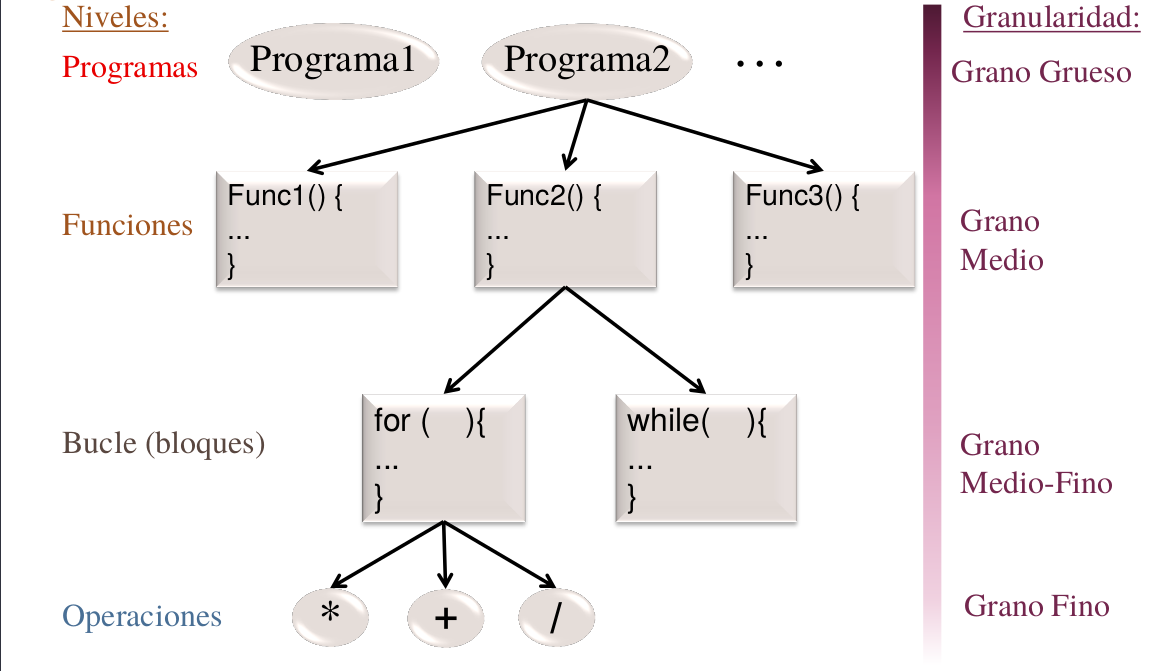
\includegraphics[scale=0.4]{paralelismo.png}
\caption{Niveles de paralelismo y granularidad}
\end{figure}
A este paralelismo que ese puede detectar en distintos niveles de un código secuencial se le denomina \emph{paralelismo funcional}.
\newpage
Por ejemplo:
\begin{listing}[H]
\begin{minted}[linenos,xleftmargin=4.5cm,xrightmargin=4.5cm]{c}
#include <stdio.h>
using namespace std;
int func1();
int func2();
int func3();
int main(){
	#pragma omp pararell sections{
		#pragma omp section
			func1();
		#pragma omp section
			func2();
		#pragma omp section
			func3();	
		}
}

\end{minted}
\caption{Paralelismo funcional}
\end{listing}

\paragraph{Paralelismo de tareas}

El \emph{paralelismo de tareas} se encuentra extrayendo de la definición de la aplicación la estructura lógica de funciones de la aplicación. En esta estruyctura, los bloques son funciones y las conexiones entre ellos reflejan el flujo de datos entre funciones. Analizando esta estructura podemos encotnrar paralelismo entre las funciones.\\
Está relacionado con el \textbf{paralelismo a nivel de función}.
\begin{figure}[H]
\centering
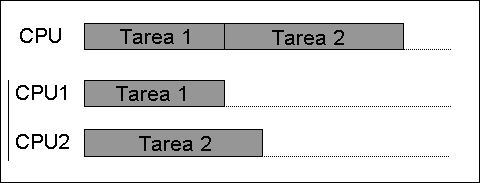
\includegraphics[scale=0.75]{paralelismo_tareas.png}
\caption{Paralelismo de tareas}
\end{figure}

\paragraph{Paralelismo de datos}

El \emph{paralelismo de datos} está relacionado con el \textbf{paralelismo a nivel de bucle}. Se encuentra implícito en las operaciones con estructuras de datos (vectores y matrices) y se puede extraer de una representación matemática de las operaciones de la aplicación. Por ejemplo, como vectores y matrices se operan mediante bucles, podremos implementarlas mediante paralelismo a nivel de bucle. Así aparece el paralelismo de datos al analizar las operaciones realizadas con la misma estructura de datos pero en distinta iteración.\footnote{Las instrucciones multimedia de los procesadores suelen acelerar el procesamiento vectorial ya que aplican la misma operación en paralelo a múltiples datos dentro de un registro.}\\
El paralelismo también se puede clasificar en función de la \emph{granularidad} o \emph{magnitud de la tarea} candidata a la paralelización. El grano más pequeño (\textit{grano fino}) se asocia generalmente al paralelismo entre operaciones o instrucciones y el \textit{grueso} al paralelismo entre programas. Entre ambos existe el \textit{grano medio}, asociado a los bloques funcionales lógicos de la aplicación.\\
Por ejemplo:
\begin{listing}[H]
\begin{minted}[linenos,xleftmargin=4.5cm,xrightmargin=4.5cm]{c}
#include <stdio.h>
using namespace std;
const int SIZE=100;
int main(){
int a[SIZE];
int b[SIZE];
int c[SIZE];
for(int i=0;i<SIZE;i++)
	a[i]=b[i]+c[i]
return 0
}
\end{minted}
\caption{Paralelismo de datos}
\end{listing}
\subsubsection{Unidades de ejecución: instrucciones, hebras y procesos}

En el nuvel superior, el sistema operativo se encarga de gestionar la ejecución de unidades de mayor granularidad (\textit{procesos} y \textit{hebras}). Cada proceso en ejecución tiene su propia región de memoria. Los sistemas operativos multihebra permiten que un proceso se componga de una o varias hebras.\\
La diferencia principal entre hebra y proceso es que una hebra tiene su propia pila y contenido de registros, entre ellos IP (\textit{Instruction Pointer}) que almacena la dirección de la siguiente instrucción a ejecutar por la hebra, pero comparte código, variables globales y otros recursos como archivos abiertos con el resto de hebras del mismo proceso. Estas características hacen que las hebras se puedan crear y destruir en menor tiempo que los procesos y que la comunicación, sincronización y conmutación entre hebras de un proceso sea más rápida que entre procesos. Esto permite que las hebras tengan una \textbf{granularidad menor que los procesos}.\\
El paralelismo implícito en el código de una aplicación se puede hacer \emph{explícito} a nivel de instrucciones, hebras, procesos o dentro de una instrucción.
\newpage
\subsubsection{Relación entre paralelismo implícito, explícito y arquitecturas paralelas}

El paralelismo se puede hacer explícito de varias formas:
\begin{enumerate}
\item El paralelismo \emph{entre programas} se utiliza a través de procesos. Cuando se ejecuta un programa, se crea su proceso asociado.
\item El paralelismo \emph{entre funciones} se puede utilizar a nivel de procesos o de hebras.
\item El paralelismo \emph{dentro de un bucle} también se puede utilizar a nivel de procesos o hebras. Además, podemos aumentar la granularidad asociando un mayor número de iteraciones a cada unidad de ejecución paralela. También se puede hacer explícito dentro de una instrucción vectorial.
\item El paralelismo \emph{entre operaciones} se puede aprovechar en arquitecturas con paralelismo a nivel de instrucción (\textit{ILP}), ejecutando en paralelo las instrucciones asociadas a las operaciones independientes.
\end{enumerate}

\begin{figure}[H]
\centering
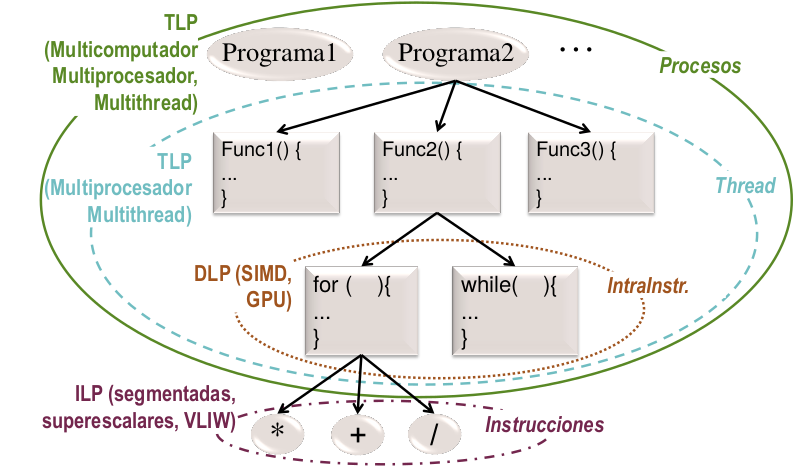
\includegraphics[scale=0.5]{paralelismo_implicito_explicito.png}
\caption{Paralelismo implícito, explícito y arquitecturas paralelas}
\end{figure}

\subsubsection{Detección, utilización, implementación y extracción de paralelismo}

En los procesadores \textit{ILP} superescalares o segmentados la arquitectura extrae paralelismo. Para ello, se eliminan dependencias de datos falsas entre instrucciones. En estos procesadores, la arquitectura extrae paralelismo \emph{implícito} en las entradas en tiempo de ejecución (\textit{dinámicamente}). El \textbf{grado de paralelismo} de las instrucciones aprovechado se puede incrementar con ayuda de \emph{compilador} y \emph{programador}. En general,\begin{definition}
El grado de paralelismo de un conjunto de entradas a un sistema es el máximo número de entradas del conjunto que se pueden ejecutar en paralelo.
\end{definition}
\begin{aclaration}
En el caso de los procesadores, las entradas son instrucciones.
\end{aclaration}
Debido a las dependencias entre entradas, este grado máximo será generalmente inferior al de entradas del conjunto. En las arquitecturas ILP VLIW \footnote{Instruction Level Parallelism Very Long Instruction Word} el paralelismo está ya \emph{explícito} en las entradas, ya que el paralelismo se determina fuera del hardware. En este caso, el análisis de dependencias es estático; el compilador es el principal responsable de extraer el paralelismo. No obstante, la ayuda de un prograamador puede incrementar el grado de concurrencia aprovechado finalmente por la arquitectura.\\
Para el compilador es difícil extraer el paralelismo, por lo que si el programador lo hace definiendo hebras y/o procesos se conseguirá mayor concurrencia.
\begin{figure}[H]
\centering
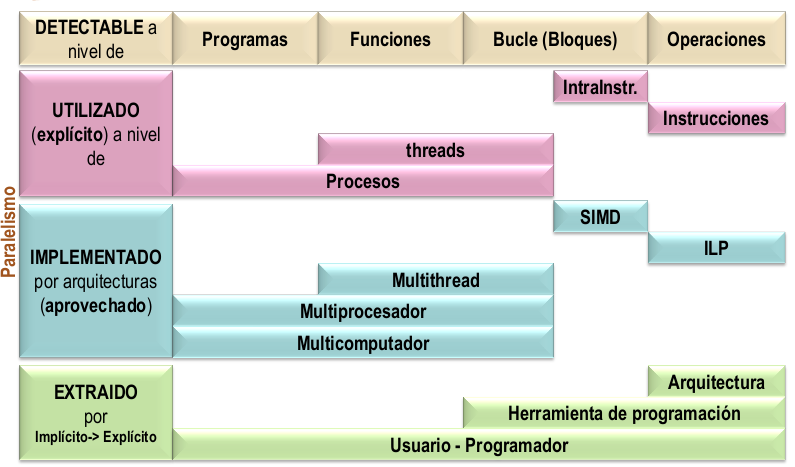
\includegraphics[scale=0.5]{deteccion_paralelismo.png}
\caption{Detección, utilización, implementación y extracción del paralelismo}
\end{figure}
\subsection{El paralelismo en las arquitecturas}
\subsubsection{Clasificaciones de las arquitecturas paralelas}
El paralelismo se ha implementado en las arquitecturas siguiendo dos líneas fundamentales. 
\begin{enumerate}
\item \textbf{Replicación de elementos}. Se incluyen unidades funcionales, procesadores, módulos de memoria, etc. entre los que se distribuye el trabajo. Ejemplos: multiprocesadores, procesadores de E/S, etc.
\item \textbf{Segmentación de cauce}. Consiste en dividir un elemento (unidad funcional, procesador, etc.) en una serie de etapas que funcionan de forma independiente y por las que pasan los operandos, instrucciones, etc. procesados por el elemento. Así, el elemento en cuestión realiza simultáneamente distintas etapas de su procesamiento.
\end{enumerate} 

La \textbf{clasificación \textit{(o taxonomía)} de Flynn} divide los computadores en cuatro clases según el número de secuencias o flujos \emph{de instrucciones} y flujos o secuencias \emph{de datos} que se pueden procesar simultáneamente en el computador.
\begin{enumerate}
\item \textbf{Computadores SISD} (\textit{Single Instruction Single Data}). Un único flujo de instrucciones genera resultados, definiendo un único flujo de datos.
\item \textbf{Computadores SIMD} (\textit{Single Instruction Multiple Data}). Un único flujo de instrucciones procesa operandos y genera resultados, defiendo varios flujos de datos, ya que cada instrucción codifica realmente varias operaciones iguales que actúan sobre operandos distintos.
\item \textbf{Computadores MIMD} (\textit{Multiple Instruction Multiple Data}). El computador ejecuta varias secuencias o flujos distintos de instrucciones y cada uno de ellos procesa operandos y genera resultados definiendo un único flujo de instrucciones, de forma que también se generan varios flujos de datos, uno por cada flujo de instrucciones.
\item \textbf{Computadores MISD} (\textit{Multiple Instruction Single Data}). Se ejecutan varios flujos distintos de instrucciones aunque todos actúan sobre el mismo flujo de datos.
\end{enumerate}

\begin{figure}[H]
\centering
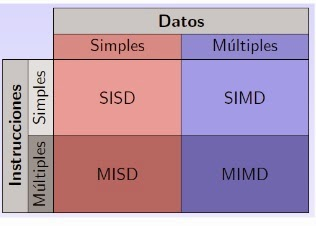
\includegraphics[scale=1]{taxonomia_flynn.png}
\caption{Taxonomía de Flynn}
\end{figure}
\paragraph{SISD}
En un computador \textbf{SISD} existe una única unidad de control que recibe las instrucciones de memoria, las decodifica y genera los códigos que definen la operación correspondiente a cada instrucción que debe realizar la unidad de procesamiento. El flujo de datos se establece a partir de los operandos necesarios para realizar la operación correspondiente (se traen de memoria) y de los resultados generados por las instrucciones (se almacenan en memoria).

\begin{figure}[H]
\centering
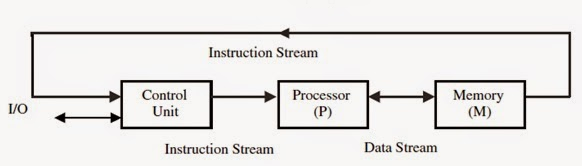
\includegraphics[scale=0.7]{sisd.png}
\caption{Arquitectura SISD}
\end{figure}

\paragraph{SIMD}

En un computador \textbf{SIMD} los códigos que genera la única unidad de control a partir de cada instrucción actúan sobre varias unidades de procesamiento distintas. De esta forma, un computador SIMD puede realizar varias operaciones similares simultáneas con operandos distintos. Cada una de las secuencias de operandos y resultados utilizados por las distintas unidades de proceso definen un flujo de datos diferente.

\begin{figure}[H]
\centering
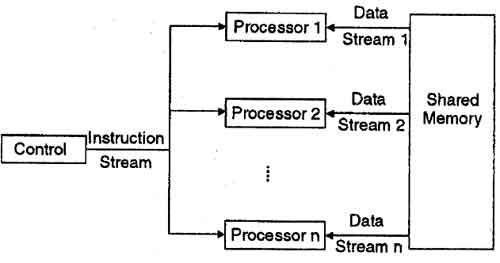
\includegraphics[scale=0.8]{simd.png}
\caption{Arquitectura SIMD}
\end{figure}

\paragraph{MIMD}

En un computador \textbf{MIMD} existen varias unidades de control que decodifican las instrucciones correspondientes a distintos programas. Cada uno de estos programas procesa conjuntos de datos diferentes, que constituyen distintos flujos de datos.

\begin{figure}[H]
\centering
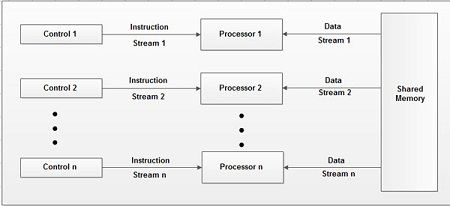
\includegraphics[scale=1]{mimd.png}
\caption{Arquitectura MIMD}
\end{figure}

\paragraph{MISD}

Los computadores \textbf{MISD} forman una clase de computadores cuyo comportamiento se puede implementear con iguales prestaciones que en un computador MIMD en el que sus procesadores se sincronizan para que los datos vayan pasando desde un procesador a otro. Por tanto, si bien existen computadores SISD (monoprocesador), SIMD (procesadores matriciales y vectoriales) y MIMD (multiprocesadores y multicomputadores), los computadores MISD específicos no existen, ya que su forma de procesamiento se puede implementar en un MIMD.

\begin{figure}[H]
\centering
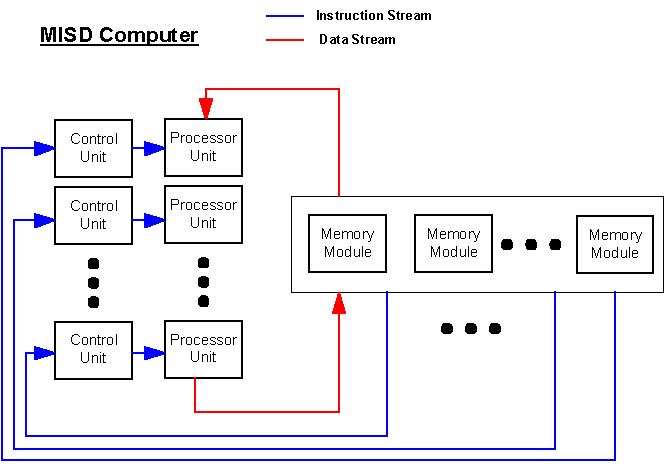
\includegraphics[scale=0.5]{misd.png}
\caption{Arquitectura MISD}
\end{figure}

La taxonomía de Flynn pone de manifiesto dos tipos de paralelismo que pueden utilizarse: paralelismo de \emph{datos} y paralelismo de \emph{instrucciones}. El de \emph{datos} ese explota cuando una misma función, instrucción, etc. se ejecuta repetidas veces en paralelo con diferentes datos. Se explota fundamentalmente en las arquitecturas \textbf{MIMD}.\\
El paralelismo \emph{funcional} se aprovecha cuando las funciones, bloques, instrucciones, etc. (iguales o distintas) que intervienen en la aplicación se ejecutan en paralelo. 

\subsection{Espacio de diseño. Clasificación y estructura general}
\subsubsection{Clasificación}
Los sistemas de paralelismo de alto nivel se han clasificado en dos grupos en función de la organización de su espacio de direcciones:
\begin{enumerate}
\item \textbf{Sistemas con memoria compartida} (SM, \textit{Shared Memory}) o simplemente \textbf{multiprocesadores}. Son sistemas en los que todos los procesadores comparten el mismo espacio de direcciones. El programador no necesita saber dónde están almacenados los datos.
\item \textbf{Sistemas con memoria distribuida} (DM, \textit{Distributed Memory}) o \textbf{multicomputadores} . Cada procesador tiene su propio espacio de direcciones. El programador necesita saber dónde están almacenados los datos.
\end{enumerate}

En un procesador SMP (\textit{Symmetric MultiProcessor}) el tiempo de acceso de los procesadores a memoria o dispositivos de E/S será igual sea cual sea la posición a la que accedan. En estos procesadores , el acceso a memoria se realiza a través de la red de interconexión.\\
En los multicomputadores, cada procesador tiene su propio módulo de memoria local al que puede acceder directamente. En esta configuración la red de interconexión se utiliza para transferir mensajes entre nodos de la red. \\

\begin{table}[H]
\centering
\begin{tabular}{|m{3cm}|m{6cm}|m{6cm}|}
\hline
\textbf{Atributo} & 
\begin{center}
\textbf{Multiprocesador SMP} 
\\
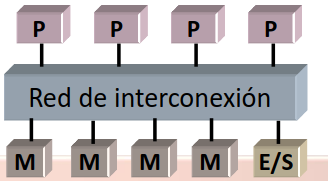
\includegraphics[scale=0.2]{multiprocesador_smp.png} 
\end{center}
& 
\begin{center}
\textbf{Multicomputador} 
\\
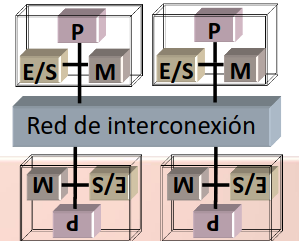
\includegraphics[scale=0.2]{multicomputador.png} 
\end{center}
\\
\hline
Espacio de direcciones & Compartido por todos los procesadores & Cada procesador tiene el suyo \\
\hline
Programador & NO necesita saber dónde están almacenados los datos & Necesita saber dónde están almacenados los datos \\
\hline
Latencia en el acceso a memoria & Grande & Pequeña \\
\hline
Comunicación & Implícita mediante variables compartidas. Datos no duplicados & Explícita mediante
software para paso de mensajes. Datos duplicados. \\
\hline
Sincronización & Necesita implantar primitivas & Mediante software de comunicación \\
\hline
Distribución de código y datos entre procesadores & No necesaria & Necesaria \\
\hline
Programación & Sencilla & Complicada \\
\hline
\end{tabular}
\caption{Diferencias entre multicomputadores y multiprocesadores}
\end{table}
\paragraph{Incremento de escalabilidad en multiprocesadores y red de interconexión}
Se han seguido varios caminos para lograrlo:
\begin{enumerate}
\item Incorporar cachés para que cada procesador disponga de una caché local, reducciendo el número de accesos a memoria.
\newpage
\item Usar redes con menor latencia y mayor ancho de banda que un bus.
\begin{enumerate}
\item Jerarquía de buses.
	\begin{figure}[H]
	\centering
	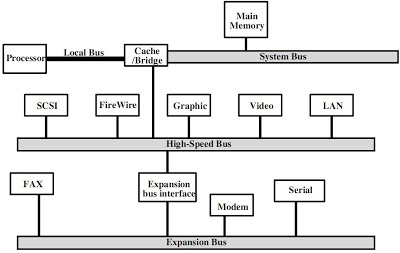
\includegraphics[scale=0.5]{jerarquia_buses.jpg}
	\caption{Jerarquía de buses}
	\end{figure}
\item Multietapa
	\begin{figure}[H]
	\centering
	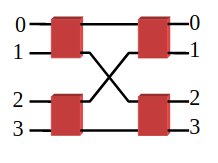
\includegraphics[scale=0.5]{multietapa.png}
	\caption{Multietapa}
	\end{figure}
\item Barras cruzadas. Proporciona el mejor rendimiento.
	\begin{figure}[H]
	\centering
	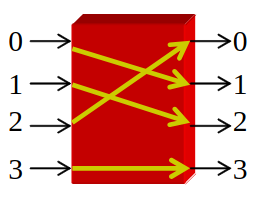
\includegraphics[scale=0.5]{barras_cruzadas.png}
	\caption{Barras cruzadas}
	\end{figure}
\end{enumerate}
\item Distribuir físicamente los módulos de memoria principal entre los procesadores manteniendo el espacio de direcciones compartido. Se pierde la propiedad de la simetría.

\end{enumerate}

A raíz de la aparición de multiprocesadores con memoria físicamente distribuida surgieron nuevas denominaciones para sistemas con múltiples procesadores. Entonces los multiprocesadores se empezaron a clasificar según la uniformidad en el acceso a memoria:
\begin{enumerate}
\item \textbf{Multiprocesadores con acceso a memoria uniforme} o UMA (\textit{Uniform Memory Access}). El tiempo de acceso de los procesadores a una determinada posición de memoria principal (o caché) es igual sea cual sea el procesador (SMP).
\item \textbf{Multiprocesadores con acceso a memoria no uniforme} o NUMA (\textit{Non-Uniform Memory Access}). El tiempo de acceso depende del procesador.
\begin{enumerate}
\item \textbf{NCC-NUMA} (\textit{Non-Cache-Coherent Non-Uniform Memory Access}) o arquitecturas con acceso a memoria no uniforme sin coherencia de caché entre nodos o, simplemente, \textbf{NUMA}. En estas arquitecturas no hay hardware para evitar incoherencias entre cachés de distintos nodos. Esto hace que los datos modificables compartidos no se pueden trasladar a caché de nodos remotos, hay que acceder individualmente a ellos a través de la red.
\item \textbf{CC-NUMA} (\textit{Cache-Coherent Non-Uniform Memory Access}) o arquitecturas con acceso a memoria no uniforme y caché coherente. Tienen hardware para mantener la coherencia de caché, pero introduce un retardo que hace que la arquitectura escale en menor grado que un NUMA.
\item \textbf{COMA} (\textit{Cache Only Memory Access}) o arquitecturas con acceso a memoria solo caché. La memoria local se gestiona como caché e incluye un hardware de mantenimiento. El coste y el retardo de estos sistemas es mayor que en CC-Numa, por lo que no existe actualmente ningún sistema comercial COMA.
\end{enumerate}
\end{enumerate}
\subsubsection{Propuesta de clasificación de arquitecturas con múltiples threads}
\begin{itemize}
\item \textbf{TLP} (\textit{Thread Level Parallelism}). Múltiples flujos de control concurrentemente o en paralelo.
\begin{itemize}
\item \textbf{Implícito}. Flujos de control creados y gestionados por la arquitectura.
\item \textbf{Explícito}. Flujos de control creados y gestionados por el Sistema Operativo.
\begin{itemize}
\item \textbf{Con una instancia SO}. Multiprocesadores, multicores y cores multithread.
\item \textbf{Con múltiples instancias SO}. Multicomputadores.
\end{itemize}
\end{itemize}
\end{itemize}
\subsection{Evolución y prestaciones de las arquitecturas}
\subsubsection{Tiempo de CPU de un programa}
Para ilustrar el proceso de evolución de las arquitecturas se utiliza una expresión que relaciona el tiempo de CPU de un programa con tres características a través de las cuales podemos extraer consecuencias importantes relacionadas con la influencia de la tecnología, el compilador y la arquitectura en las prestaciones:
\begin{equation}
T_{tarea}=NI \cdot CPI \cdot T_{ciclo}=NI \cdot \frac{CPI}{f}
\end{equation}
\[
T_{ciclo}=\frac{1}{f}
\]
donde $T_{tarea}$ es el tiempo de CPU de un programa (también se puede notar como $T_{CPU}$), $NI$ es el número de instrucciones mñaquina del programa, $CPI$ es el número medio de ciclos por instrucción y $T_{ciclo}$ el período de reloj del procesador (inverso de la frecuencia, $f$). EL valor de CPI se puede expresar como:
\newpage
\begin{equation}
CPI=\frac{Ciclos_{programa}}{NI}=\frac{\sum_{i=1}^{n} CPI_{i} \cdot I_i}{NI}
\end{equation}
\[
Ciclos_{programa}=\sum_{i}^{n}CPI_i \cdot I_i
\]
donde $CPI_{i}$ es el número medio de ciclos de las instrucciones de tipo $i$ y $NI_{i}$ es el número de instrucciones de ese tipo.\\
Uno de los objetivos fundamentales en el diseño de un computador es reducir el tiempo de ejecución de los programas ($T_{tarea}$).\\
La ecuación (1) puede ayudarnos a comprender, por ejemplo, la diferencia entre RISC y CISC:
\begin{itemize}
\item En \textbf{CISC} se opta por reducir el $NI$ para reducir $T_{CPU}$, aunque aumenta el $CPI_i$. Sin embargo, este aumento se puede contrarrestar mejorando la frecuencia del procesador ($f$).
\item En \textbf{RISC} se opta por reducir el $CPI_i$ y aumentar el $NI_i$. Al igual que en el caso anterior, el aumento de $NI_i$ se puede contrarrestar mejorando $f$.
\end{itemize}
Hay procesadores que pueden emitir (mandar a ejecutar) varias instrucciones al mismo tiempo. En ese caso:
\[\frac{CPE}{IPE}=CPI\] 	
\begin{equation}
T_{CPU}=NI \cdot \frac{CPE}{IPE} \cdot T_{ciclo}
\end{equation}
donde $CPE$ es el número mínimo de ciclos transcurridos entre los instantes en los que el procesador puede emitir instrucciones y $IPE$ es el número de instrucciones que pueden emitirse en un instante.\\
También hay procesadores que pueden codificar varias operaciones en una instrucción:
\[NI=\frac{N_{operaciones}}{Operaciones_{instruccion}}\]
\begin{equation}
T_{CPU}=\frac{N_{operaciones}}{Operaciones_{instruccion}} \cdot CPI \cdot T_{ciclo}
\end{equation}
donde $N_{operaciones}$ es el número de operaciones que realiza el programa y $Operaciones_{instruccion}$ el número de operaciones que puede codificar una instrucción.
\begin{figure}[H]
\centering
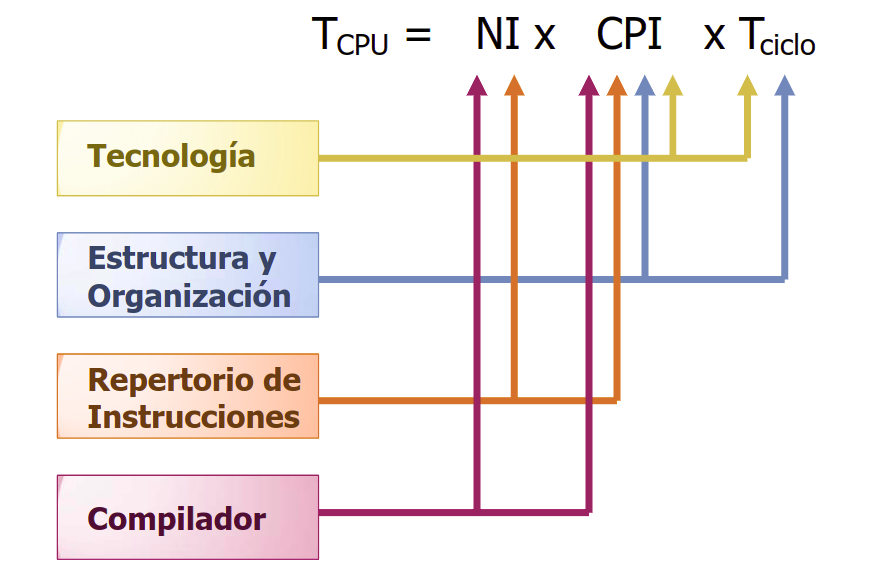
\includegraphics[scale=0.25]{optimizacion_t_cpu.png}
\caption{Optimizaciones del tiempo de CPU y sus causantes}
\end{figure}
\subsubsection{Medidas de productividad: MIPS y MFLOPS}
El tiempo de respuesta, la productividad y la funcionalidad se pueden englobar en una única medida de prestaciones, conocida como \emph{tiempo de respuesta para una entrada compleja}. Corresponde a una secuencia representativa de entradas elementales del sistema. En esta línea están los \emph{MIPS} y los \emph{MFLOPS}.
\paragraph{MIPS (Millions of Instructions Per Second)}
Vienen determinados por la siguiente fórmula:
\[T_{CPU}=NI \cdot CPI \cdot T_{ciclo} \]
\[f=\frac{1}{T_{ciclo}} \]
\begin{equation}
MIPS=\frac{NI}{T_{CPU} \cdot 10^6}=\frac{f}{CPI \cdot 10^6}
\end{equation}
Como podemos ver, esta medida puede variar según el programa, por lo que no sirve como medida característica de una máquina. Además, depende del repertorio de instrucciones, por lo que no permite comparar máquinas con repertorios distintos. Por último, puede ser inversamente proporcional a las prestaciones, ya que aquel programa que utilice más instrucciones tendrá más MIPS, indicando erróneamente que es mejor.
\subparagraph{\boldmath $MIPS_{pico}$}
Es el máximo valor téórico de MIPS para una arquitectura. Se calcula mediante la siguiente fórmula:
\begin{equation}
MIPS_{pico}=\frac{f \cdot IPC_{max}}{10^6}
\end{equation}
donde $IPC_{max}$ representa el número máximo de operaciones por ciclo que puede realizar la arquitectura.
\paragraph{MFLOPS (Millions of FLoating point Operations Per Second)}
Vienen definidos por:
\begin{equation}
MFLOPS=\frac{Operaciones_{coma flotante}}{T_{CPU} \cdot 10^6}
\end{equation}
Por un lado no es una medida adecuada para todos los programas, ya que solo tiene en cuenta las operaciones en coma flotante. Además, el conjunto de operaciones en coma flotante no es el mismo en todas las máquinas, así como el coste por operación. Para resolver este último problema, se utilizan a veces los MFLOPS normalizados, que se obtienen dando un peso relativo a cada instrucción.
\subparagraph{\boldmath $MFLOPS_{pico}$}
Se calculan mediante la siguiente expresión:
\begin{equation}
MFLOPS_{pico}=\frac{f \cdot \text{Operaciones en coma flotante/ciclo}_{max}}{10^6}
\end{equation}
\subsubsection{Conjuntos de programas de prueba (\textit{benchmarks})}

Para evaluar una arquitectura hay que considerar tanto las medidas de prestaciones que caracterizan a la arquitectura como las medidas de prestaciones que permiten comparar arquitecturas con \emph{igual uso}.\\
Para ello, se definen conjuntos de programas de prueba (\textit{benchmarks}) representativos de todos los posinlrd programas, representando la carga de trabajo usual en la máquina que los ejecutará. Hay de varios tipos:
\begin{enumerate}
\item \textbf{Aplicaciones reales}. Presentan problemas en cuanto a la portabilidad. Ejemplos: SPEC CPU2006
\item \textbf{Núcleos o \textit{kernels}}. Programas que evalúan una característica concreta. Resolución de sistemas de ecuaciones, multiplicación de matrices, etc.
\item \textbf{Programas de pruebas simples (\textit{toys})}. Son pequeños y fáciles de escribir. Test ping-pong, evaluación de operaciones con enteros y flotantes, etc.
\item \textbf{Programas sintéticos}. Dhrystone, Whetstone, etc. No realizan ninguna tarea concreta.
\item \textbf{Aplicaciones diseñadas}. Predicción del tiempo, simulación de terremotos, etc.
\subsubsection{Ganancia en prestaciones}
Si incrementamos las prestaciones de un computador mejorando alguno de sus recursos o elementos, podremos utilizar la \emph{ganancia} para evaluar hasta qué punto una mejora de prestaciones es \textit{p} veces mayor o menor que antes.\\
Este aumento de prestaciones se expresa mediante la ganancia de velocidad ($S_p$, \textit{Speed Up})
\begin{equation}
S_p=\frac{T_1}{T_p}=\frac{V_p}{V_1}
\end{equation}
donde:
\begin{itemize}
\item $V_1$ es la velocidad de la máquina base.
\item $V_p$ es la velocidad de la máquina mejorada.
\item $T_1$ es el tiempo de ejecución en la máquina base.
\item $T_p$ es el tiempo de ejecución en la máquina mejorada.
\end{itemize}
\end{enumerate}

Surge la cuestión de hasta qué punto la mejora en un factor \emph{p} se pone de manifiesto en la mejora final objetiva, surgiendo así la \textbf{Ley de Amdahl}.
\begin{law}[de Amdahl]
La mejora de velocidad, $S_p$ que se puede obtener al mejorar un recurso de una máquina en un factor $p$ está limitada por la expresión:
\[ S_p \leq \frac{p}{1 + f \cdot (p-1)} \]
\end{law}
donde $f$ es el porcentaje de operaciones que realiza la máquina en las que no se pone de manifiesto la mejora (por supuesto, $0 \leq f \leq 1$). Así, solo si $f=0$ (la mejora se utiliza siempre) una mejora de factor $p$ en un elemento se observa n la misma medida en la máquina.
\subparagraph{Ejemplo}
Si un programa pasa un $25\%$ del tiempo de ejecución realizando operaciones de coma flotante y mejoramos la máquina haciendo que esas instrucciones se ejecuten en la mitad de tiempo ($p=2$);
\[ S_p \leq \frac{2}{1 + 0.75 \cdot (2-1)} \leq \frac{2}{1.75} \leq 1.14\]
Es decir, la mejora en la arquitectura completa será de sólo un $14\%$.
\subsection{Ejercicios}
\begin{enumerate}
\item Calcule los $MIPS_{pico}$ de una arquitectura con una CPU superescalar con un IPC de 3 instrucciones por ciclo y una frecuencia de 2Ghz.
\begin{solution}
\[ MIPS_{pico}=\frac{2 \cdot 10^9 ciclos/seg \cdot 3 instrucciones/ciclo}{10^6}=6 \cdot 10^3 \ MIPS \simeq 6 \ GIPS \]
\end{solution}
\item En el  código de  prueba  (benchmark) que  ejecuta un procesador  no  segmentado  que  funciona a 300  MHz,  hay  un  20\%  de  instrucciones  LOAD  que  necesitan  4  ciclos,  un  10\%  de  instrucciones  STORE  que necesitan  3  ciclos,  un  25\%  de  instrucciones  con  operaciones  de  enteros  que  necesitan  6  ciclos,  un  15\%  de instrucciones  con  operandos  en  coma  flotante  que  necesitan  8  ciclos  por  instrucción,  y  un  30\%  de instrucciones de salto que necesitan 3 ciclos. 
\begin{enumerate}
\item ¿Cuál es la ganancia que se puede obtener por reducción a 3 ciclos de las instrucciones con enteros?
\item ¿Cuál es la ganancia que se puede obtener por reducción a 3 ciclos de las instrucciones en coma flotante?
\end{enumerate}
\begin{solution}
\begin{table}[H]
\centering
\begin{tabular}{|c|c|c|}
\hline
\textbf{Instrucción} & \textbf{Porcentaje de uso} & \textbf{CPI} \\
\hline
LOAD & 20\% & 4 \\
\hline
STORE & 10\% & 3 \\
\hline
Operaciones con enteros & 25\% & 6 \\
\hline
Operaciones en coma flotante & 15\% & 8 \\
\hline
Salto & 30\% & 3 \\
\hline
\end{tabular}
\par
\bigskip
Antes de la optimización
\end{table}
\newpage
\begin{itemize}
\item Apartado a)
\begin{table}[H]
\centering
\begin{tabular}{|c|c|c|}
\hline
\textbf{Instrucción} & \textbf{Porcentaje de uso} & \textbf{CPI} \\
\hline
LOAD & 20\% & 4 \\
\hline
STORE & 10\% & 3 \\
\hline
Operaciones con enteros & 25\% & \textst{6} 3 \\
\hline
Operaciones en coma flotante & 15\% & 8 \\
\hline
Salto & 30\% & 3 \\
\hline
\end{tabular}
\par
\bigskip
Tras la optimización
\end{table}
Como el CPI de las operaciones con enteros se reduce a la mitad, $p=2$.\\
Aplicamos la ley de Amdahl:
\[ S_p=\frac{p}{1 + f \cdot (p-1)} \rightarrow S_p = \frac{2}{1 + 0.75 \cdot (2-1)}= \frac{2}{1.75} \simeq  1.143 \]
\begin{center}
Por tanto la mejora será de aproximadamente el $14,3\%$
\end{center}
\item Apartado b)

\begin{table}[H]
\centering
\begin{tabular}{|c|c|c|}
\hline
\textbf{Instrucción} & \textbf{Porcentaje de uso} & \textbf{CPI} \\
\hline
LOAD & 20\% & 4 \\
\hline
STORE & 10\% & 3 \\
\hline
Operaciones con enteros & 25\% & 6 \\
\hline
Operaciones en coma flotante & 15\% & \textst{8} 3 \\
\hline
Salto & 30\% & 3 \\
\hline
\end{tabular}
\par
\bigskip
Tras la optimización
\end{table}
Como el CPI de las operaciones en coma flotante pasa de 8 a 3, $p=\frac{8}{3}=2.67$.
Aplicamos la Ley de Amdahl
\[S_p=\frac{p}{1 + f \cdot (p-1)} \rightarrow S_p=\frac{2.67}{1 + 0.85 \cdot (2.67-1)}=\frac{2,67}{1.4195} \simeq 1.88
\]
Por tanto, la mejora es aproximadamente del $88\%$

\end{itemize}

\end{solution}
\item En  un  procesador  sin  segmentación  de  cauce,  determine  cuál  de  estas  dos  alternativas  para realizar un salto condicionales mejor:
\begin{enumerate}
\item Una instrucción COMPARE actualiza un código de condición y es seguida por una instrucción BRANCH que comprueba esa condición.Se usan dos intrucciones.
\begin{table}[H]
\centering
\begin{tabular}{|c|c|c|}
\hline
\textbf{Instrucción} & \textbf{NI} & \textbf{CPI} \\
\hline
COMPARE & $0.2NI_1$ & 4 \\
\hline
Resto & $0.8NI_1$ & 3 \\
\hline
& $NI_1$ & \\
\hline
\end{tabular}
\end{table}
\item Una sola instrucción incluye la funcionalidad de las instrucciones COMPARE y BRANCH.Se usa una única instrucción.
\begin{table}[H]
\centering
\begin{tabular}{|c|c|c|}
\hline
\textbf{Instrucción} & \textbf{NI} & \textbf{CPI} \\
\hline
COMPARE + BRANCH & $0.2NI_1$ & 4 \\
\hline
Resto & $0.8NI_1-0.2NI_1=0.6NI_1$ & 3 \\
\hline
& $0.8NI_1$ & \\
\hline
\end{tabular}
\end{table}
\end{enumerate}
Hay que tener en cuenta que hay un 20\% de instrucciones BRANCH para a) en el conjunto de programas de prueba; que las instrucciones BRANCH en a) y COMPARE+BRANCH en b) necesitan 4  ciclos mientras que todas las demás necesitan sólo 3; y que el ciclo de reloj de la a) es un 25\% menor que el de la b), dado que en  éste caso la mayor funcionalidad de la instrucción COMPARE+BRANCH ocasiona una mayor complejidad en el procesado.
\begin{solution}
\textbf{Considero que en el apartado a) la instrucción BRANCH entra en el resto, por lo que consume 3 CPI.}\\
Sabemos que $T_{ciclo1}=0.75 \cdot T_{ciclo2} \rightarrow T_{ciclo2}=1.33 \cdot T_{ciclo1}$
Ahora calculamos los $T_{CPU}$. Para ello, comenzamos por los $CPI_i$
\begin{itemize}
\item $CPI_1=\frac{0.2\cdot NI_1}{NI_1} \cdot 4 + \frac{0.8 \cdot NI_1}{NI_1} \cdot 3 = 3.2$ 
\item $T_{CPU1}=NI_1 \cdot CPI_1 \cdot T_{ciclo1}= 3.2 \cdot NI_1 \cdot T_{ciclo1}$
\item $CPI_2=\frac{0.2\cdot NI_1}{0.8 \cdot NI_1} \cdot 4 + \frac{0.6 \cdot NI_1}{0.8 \cdot NI_1} \cdot 3 = 3.25$ 
\item $T_{CPU2}=0.8 \cdot NI_1 \cdot 3.25 \cdot 1.33 \cdot T_{ciclo1}= 3.45 \cdot NI_1 \cdot T_{ciclo1}$
\end{itemize}
Como $T_{CPU1} < T_{CPU2} $, la mejor opción es la \textbf{a)}.

\end{solution}
\item ¿Qué ocurriría en el ejercicio anterior si el ciclo de reloj fuese únicamente un 10\% mayor para b) ?
\begin{solution}
El problema nos indica que $T_{ciclo2}=1.1T_{ciclo1}$
\[T_{CPU1}=3.2 \cdot NI_1 \cdot T_{ciclo1}\]
\[T_{CPU2}=(0.8 \cdot 3.25 \cdot 1.1)NI_1 \cdot T_{ciclo1}=2.86 \cdot NI_1 \cdot T_{ciclo1}\]
En este caso, $T_{ciclo2} < T_{ciclo1}$, por lo que la opción \textbf{b)} se convierte en la mejor.
\end{solution}
\item Considere un procesador no segmentado con una arquitectura de tipo LOAD/STORE en la que las operaciones   sólo   utilizan   como   operandos   registros   de   la   CPU.   Paraun   conjunto   de   programas representativos de su actividad se tiene que el 43\% de las instrucciones son operaciones con la ALU (3 CPI), el 21\% LOADs (4 CPI), el 12\% STOREs (4 CPI) y el 24\% BRANCHs (4 CPI).Se ha podido comprobar que un 25\% de las operaciones con la ALU utilizan operandos en registros que no se vuelven  a  utilizar. Compruebe  si  mejorarían  las  prestaciones si,  para  sustituir  ese  25\%  de  operaciones,se añaden instrucciones con un dato en un registro y otro en memoria. Tengan en cuenta en la comprobación que para estas nuevas instrucciones el valor de CPI es 4 y que añadirlas ocasiona un incremento de un ciclo en el CPI de los BRANCHs, pero no afectan al ciclo de reloj.

\begin{table}[H]
\centering
\begin{tabular}{|c|c|c|}
\hline
\textbf{Instrucción} & \textbf{NI} & \textbf{CPI} \\
\hline
ALU (R-R) & $0.43NI_1$ & 3 \\
\hline
LOAD & $0.21NI_1$ & 4 \\
\hline
STORE & $0.12NI_1$ & 4 \\
\hline
BRANCH & $0.24NI_1$ & 4 \\
\hline
& $NI_1$ & \\
\hline
\end{tabular}
\caption*{Antes de la mejora}
\end{table}
\begin{solution}
\begin{table}[H]
\centering
\begin{tabular}{|c|c|c|}
\hline
\textbf{Instrucción} & \textbf{NI} & \textbf{CPI} \\
\hline
ALU (R-R) & $0.75 \cdot 0.43NI_1=0.3225NI_1$ & 3 \\
\hline
ALU (R-M) & $0.25 \cdot 0.43NI_1=0.1075NI_1$ & 4 \\
\hline
LOAD & $0.21NI_1 - 0.25 \cdot 0.43NI_1=0.1025NI_1$ & 4 \\
\hline
STORE & $0.12NI_1$ & 4 \\
\hline
BRANCH & $0.24NI_1$ & \textst{4} 5 \\
\hline
& $0.8925NI_1$ & \\
\hline
\end{tabular}
\caption*{Tras la mejora}
\end{table}
Calulamos el tiempo de CPU de ambas situaciones:
\[CPI_1=\frac{0.43NI_1}{NI_1}\cdot 3 + \frac{0.21NI_1}{NI_1} \cdot 4 + \frac{0.12NI_1}{NI_1} \cdot 4 + \frac{0.24NI_1}{NI_1} \cdot 4 = 3.57\]
\[T_{CPU1}=CPI_1 \cdot NI_1 \cdot T_{ciclo1}= 3.57NI_1 \cdot T_{ciclo1} \]

\[CPI_2=\frac{0.3225NI_1}{0.8925NI_1}\cdot 3 + \frac{0.1075NI_1}{0.8925NI_1} \cdot 4 + \frac{0.21NI_1}{0.8925NI_1} \cdot 4 + \frac{0.12NI_1}{0.8925NI_1} \cdot 4 + \frac{0.24NI_1}{0.8925NI_1} \cdot 4 = 3.91\]
\[T_{CPU2}=3.91 \cdot 0.8925NI_1 \cdot T_{ciclo2}= 3.49NI_1 \cdot T_{ciclo1} \]
Como $T_{CPU2}<T_{CPU1}$; la mejora \textbf{es efectiva}.
\end{solution}
\newpage
\item Se  ha  diseñado un compilador para la máquina LOAD/STORE del problema anterior. Ese compilador puede reducir en un 50\% el número de operaciones con la ALU, pero no reduce el número de LOADs, STOREs y BRANCHs. Suponiendo que la  frecuencia de reloj es de 50 Mhz. ¿Cuál es el número de MIPS y el tiempo de   ejecución que se consigue con el código optimizado? Compárelos con los correspondientes del código no optimizado.
\begin{table}[H]
\centering
\begin{tabular}{|c|c|c|}
\hline
\textbf{Instrucción} & \textbf{NI} & \textbf{CPI} \\
\hline
ALU (R-R) & $0.43NI_1$ & 3 \\
\hline
LOAD & $0.21NI_1$ & 4 \\
\hline
STORE & $0.12NI_1$ & 4 \\
\hline
BRANCH & $0.24NI_1$ & 4 \\
\hline
& $NI_1$ & \\
\hline
\end{tabular}
\caption*{Antes de la mejora}
\end{table}
\begin{solution}

\begin{table}[H]
\centering
\begin{tabular}{|c|c|c|}
\hline
\textbf{Instrucción} & \textbf{NI} & \textbf{CPI} \\
\hline
ALU (R-R) & $\frac{0.43NI_1}{2}$ & 3 \\
\hline
LOAD & $0.21NI_1$ & 4 \\
\hline
STORE & $0.12NI_1$ & 4 \\
\hline
BRANCH & $0.24NI_1$ & 4 \\
\hline
& $0.785NI_1$ & \\
\hline
\end{tabular}
\caption*{Tras la mejora}
\end{table}

Comenzamos calculando el Tiempo de CPU
\[
CPI_1=\frac{0.43NI_1}{NI_1}\cdot 3 + \frac{0.21NI_1}{NI_1}\cdot 4 + \frac{0.12NI_1}{NI_1}\cdot 4 + \frac{0.24NI_1}{NI_1}\cdot 4 =3.57
\]
\[
CPI_2=\frac{\frac{0.43NI_1}{2}}{0.785NI_1}\cdot 3 + \frac{0.21NI_1}{0.785NI_1}\cdot 4 + \frac{0.12NI_1}{0.785NI_1}\cdot 4 + \frac{0.24NI_1}{0.785NI_1}\cdot 4 =3.726
\]
\[T_{CPU1}=NI_1 \cdot T_{ciclo} \cdot CPI_1=3.57 \cdot NI_1 \cdot T_{ciclo}
\]
\[T_{CPU2}=0.785NI_1  \cdot CPI_2 \cdot T_{ciclo}=0.785NI_1 \cdot 3.726 \cdot T_{ciclo}=2.925 \cdot T_{ciclo}
\]
Ahora, calculamos MIPS
\begin{adjustbox}{width=\textwidth,totalheight=\textheight,keepaspectratio}
$MIPS_1=\frac{NI_1}{T_{CPU1} \cdot 10^6}=\frac{NI_1}{NI_1 \cdot CPI_1 \cdot T_{ciclo} \cdot 10^6}=\frac{f}{CPI_1 \cdot 10^6}=\frac{50 ciclos/segundo \cdot 10^6}{3.57 ciclos/instruccion \cdot 10^6}=14.005 MIPS
$
\end{adjustbox}
\begin{adjustbox}{width=\textwidth,totalheight=\textheight,keepaspectratio}
$MIPS_2=\frac{0.785NI_1}{T_{CPU2} \cdot 10^6}=\frac{NI_1}{0.785NI_1 \cdot CPI_2 \cdot T_{ciclo} \cdot 10^6}=\frac{f}{CPI_2 \cdot 10^6}=\frac{50 ciclos/segundo \cdot 10^6}{3.726 ciclos/instruccion \cdot 10^6}=13.42 MIPS
$
\end{adjustbox}
\par
La configuración 2 tiene un tiempo de CPU \textbf{mejor}. Sin embargo, si miramos la productividad, vemos como es \textbf{peor}. Esto se debe a que el sistema es más rápido, pero menos productivo, ya que la mejora se ha implementado en la parte que menos se usa.
\end{solution}
\end{enumerate}

\section{Tema 2}

\subsection{Programación paralela}

La programación paralela introduce un conjunto de problemas para el programador: división del trabajo en unidades independientes (tareas), sincronización, comunicación, etc.\\

Actualmente, las herramientas y métodos para facilitar el desarrollo de aplicaciones paralelas existentes son un activo campo de investigación. Para el programador lo más sencillo es utilizar compiladores capaces de extraer paralelismo automáticamente. Sin embargo, estos compiladores no generan código eficiente para todos los programas. Por tanto, no sirven de mucho.\\


\subsubsection{Punto de partida}

Cuando se plantea obtener una versión paralela de una aplicación, podemos utilizar como punto inicial un código secuencial que resuelva el problema para implantar el paralelismo sobre él. La principal ventaja de esta opción es la posibilidad de medir el tiempo en cada sección, permitiendo distribuir el trabajo de forma equilibrada.\\

Otra posibilidad es partir de la definición de una aplicación y buscar a partir de ella una descripción que admita paralelización.\\

Para facilitar el trabajo podemos apoyarnos en programas paralelos que aprovechen las características de la arquitectura. Si disponemos de un programa paralelo que resuelve un problema parecido en una arquitectura, podemos fijarnos en él para diseñar el nuestro.

\subsubsection{Modos de programación}

\paragraph{SPMD (paralelismo de datos)}
Todos los códigos que se ejecutan en paralelo se obtienen compilando el mismo programa. Cada copia trabaja con un conjunto de datos distintos y se ejecuta en un procesador diferente.

\paragraph{MPMD} 
Los códigos que se ejecutan en paralelo se obtienen compilando programas independientes, es decir, la aplicación principal se divide e unidades independientes. Cada unidad trabaja con un conjunto de ddatos y es asignada a un procesador.\\

SPMD es recomendable en sistemas masivamente paralelos, ya que es muy difícil encontrar cientos de unidades de código diferentes dentro de una aplicación, siendo más fácil escribir un sólo programa. En la práctica es el más utilizado en multiprocesadores y multicomputadores.

\begin{figure}[H]
\centering
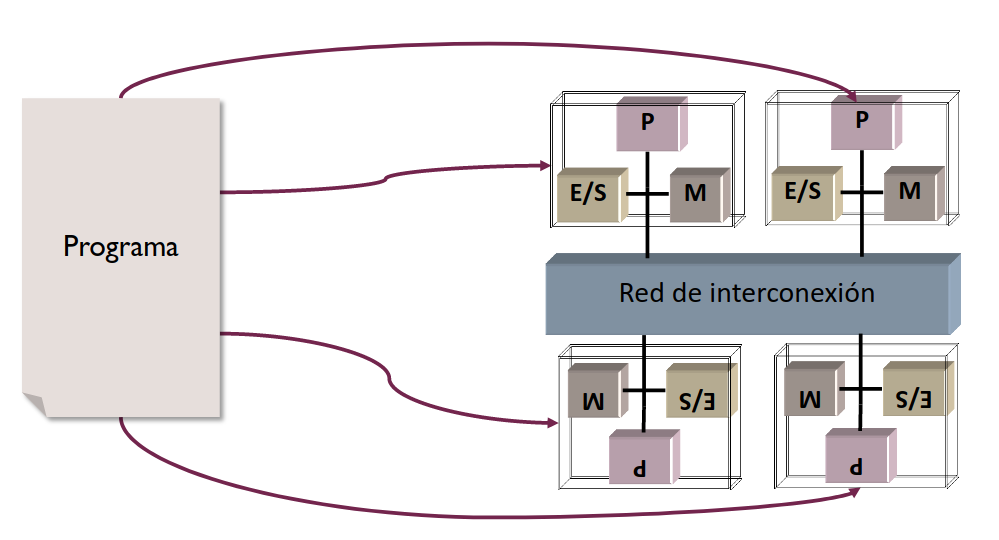
\includegraphics[scale=0.4]{spmd.png}
\caption{SPMD (Single Program Multiple Data).}
\end{figure}

\begin{figure}[H]
\centering
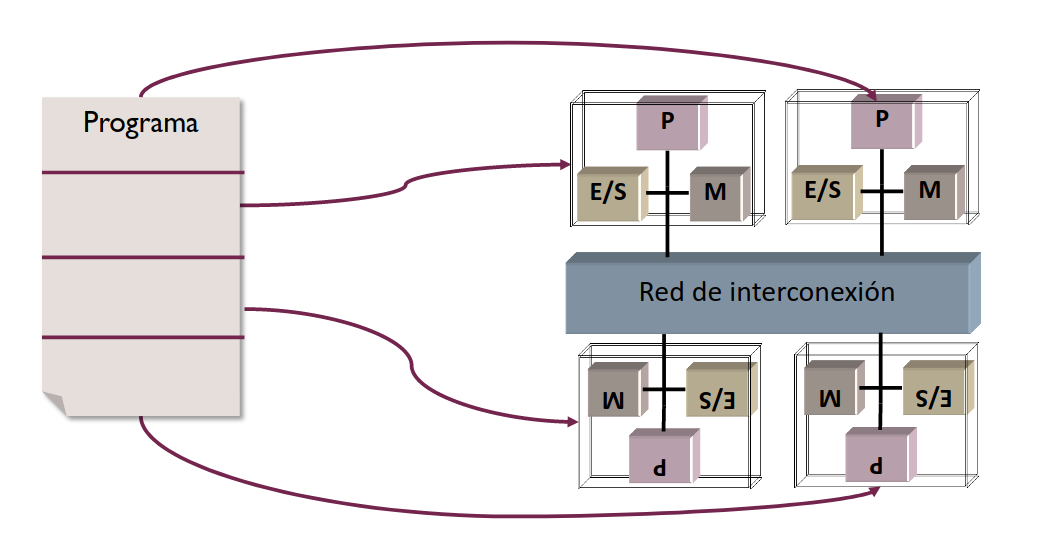
\includegraphics[scale=0.4]{mpmd.png}
\caption{MPMD (Multiple Program Multiple Data).}
\end{figure}

\subsubsection{Herramientas para obtener programas paralelos}

Las herramientas para obtener programas paralelos deben permitir de forma explícita (el trabajo lo hace el programador) o implícita (el trabajo lo hace la propia herramienta) las siguientes tareas:

\begin{itemize}
	\item Localizar paralelismo.
	\item Crear y terminar procesos.
	\item Distribuir trabajo entre procesos.
	\item Comunicación y sincronización entre procesos.
	\item Asignación de procesos a procesadores.
\end{itemize}

Para obtener un programa paralelo tenemos varias opciones:

\paragraph{Bibliotecas de funciones para programación paralela}

En esta alternativa el programador utiliza un lenguaje secuencial y una biblioteca de funciones. El cuerpo de los procesos y hebras se escribe con lenguaje secuencial y el programador se encarga explícitamente de dividir las tareas entre los procesos, crear o destruir los procesos, implementar la comunicación, etc. Las principales ventajas de esta alternativa son:
\begin{itemize}
	\item Los programadores no tienen que aprender un nuevo lenguaje.
	\item Las bibliotecas están disponibles para todos los sistemas paralelos.
	\item Las bibliotecas están más cercanas al hardware y dan al programador un control a más bajo nivel.
	\item Se pueden utilizar a la vez bibliotecas para programar con hebras y bibliotecas para programar con procesos.
\end{itemize}

Las APIs más famosas son MPI, OpenMP, Pthread, etc.

\paragraph{Lenguajes paralelos y directivas del compilador}

Sitúan al programador en un nivel de abstracción superior, ahorrando o facilitando el trabajo de paralelización, aunque puede que sólo se aproveche uno de ellos: de datos o de tareas. Los lenguajes paralelos facilitan estas tareas mediante:
\begin{itemize}
	\item Construcciones propias del lenguaje. Pueden tanto distribuir la carga de trabajo como crear y terminar procesos e incluir sincronización.
	\item Directivas del compilador.
	\item Funciones de biblioteca. Implementan en paralelo algunas operaciones usuales.
\end{itemize}

La ventaja principal de los lenguajes paralelos es que son más fáciles de escribir y entender a la vez que más cortos.

\paragraph{Compiladores paralelos}

Se pretende que un compilador paralelo extraiga automáticamente el paralelismo tanto a nivel de bucle (paralelismo de datos) como a nivel de función (paralelismo de tareas). Para ello, hacen análisis de dependencias entre bloques de código, iteraciones de un bucle o funciones. Las dependencias que detecta son RAW, WAW y WAR.\\

Los compiladores paralelos están aún limitados a aplicaciones que exhiben un paralelismo regular, como los cálculos a nivel de bucle.

\begin{figure}[H]
\centering
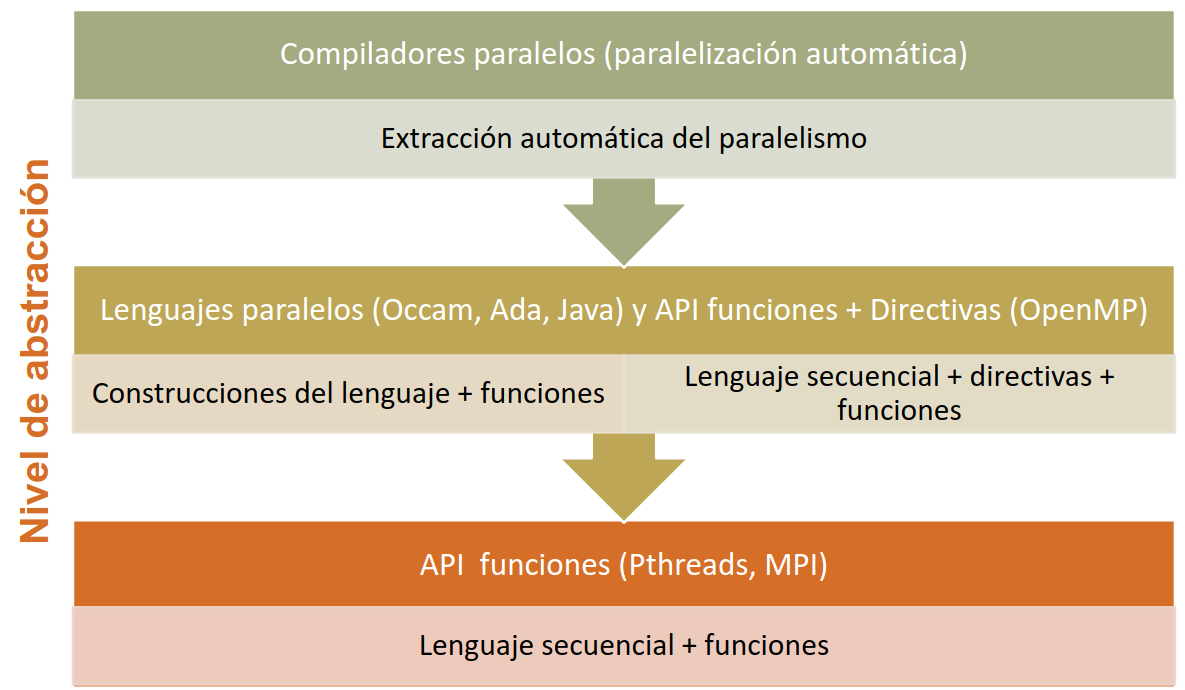
\includegraphics[scale=0.4]{herramientas_programacion_paralela.png}
\caption{Principales herramientas de programación paralela.}
\end{figure}

\paragraph{Otras alternativas}

\subparagraph{Comunicación múltiple uno a uno}
Hay componentes del grupo que envían un único mensaje (dato o estructura de datos) y componentes que reciben un único lenguaje.\\

Si todos los componentes envían y reciben, se implementa una \emph{permutación}. Algunos ejemplos de permutaciones son la rotación, el intercambio, los barajes, etc.

\begin{figure}[H]
\centering
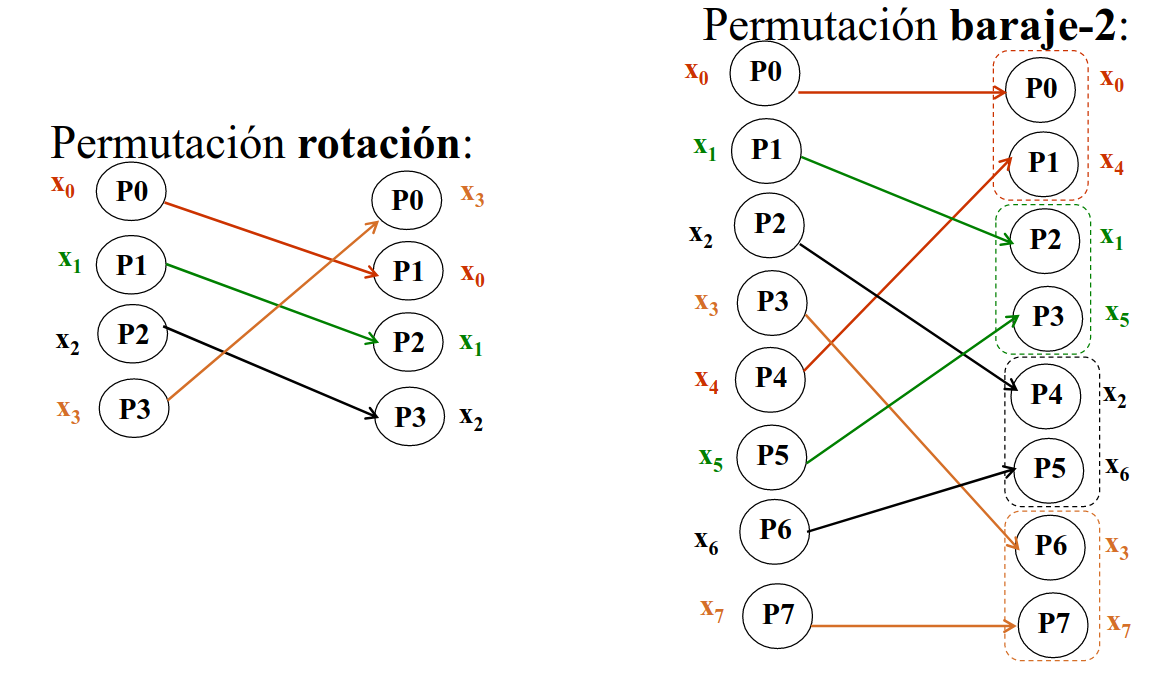
\includegraphics[scale=0.3]{uno_a_uno.png}
\caption{Comunicación uno a uno.}
\end{figure}

\subparagraph{Comunicación uno a todos}


Un proceso envía y todos los procesos reciben. Hay variantes en las que el proceso que envía no forma parte del grupo y otras en las que reciben todos excepto el que envía. Hay dos subtipos:

\begin{itemize}
	\item \textbf{Difusión}. Todos los procesos reciben el mismo mensaje.
	\item \textbf{Dispersión (\textit{scatter})}. Cada proceso receptor recibe un mensaje diferente.	
\end{itemize}

\begin{figure}[H]
\centering
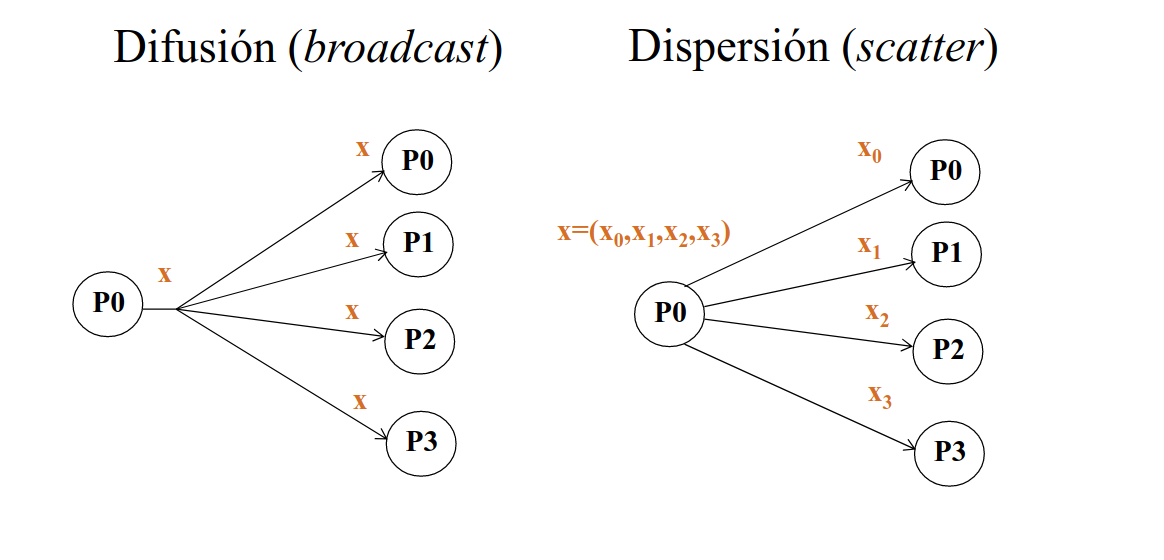
\includegraphics[scale=0.3]{uno_a_todos.png}
\caption{Comunicación uno a todos.}
\end{figure}


\subparagraph{Comunicación todos a uno}

Todos los procesos del grupo envían un mensaje a un único proceso.

\begin{itemize}
	\item \textbf{Reducción}. Los mensajes enviados por los procesos se combinan en un solo mensaje mediante algún operador. La combinación es normalmente conmutativa y asociativa.
	\item \textbf{Acumulación (\textit{gather})}. Los mensajes se reciben de forma concatenada en el receptor. El orden en que se concatenan depende normalmente del identificador de proceso.
\end{itemize}

\begin{figure}[H]
\centering
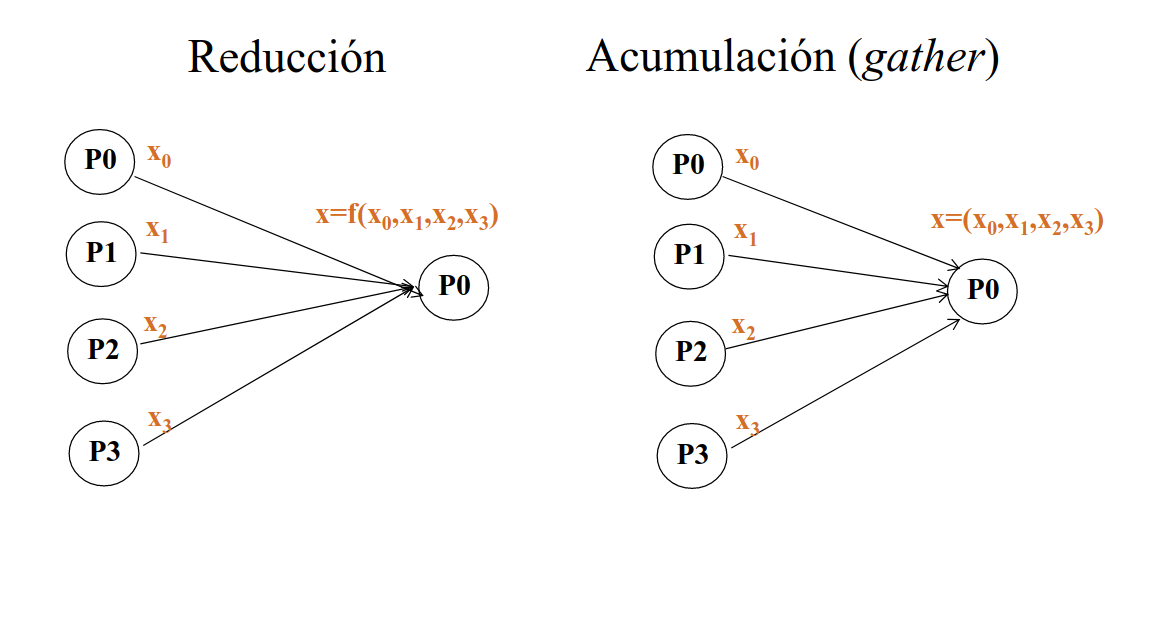
\includegraphics[scale=0.3]{todos_a_uno.png}
\caption{Comunicación todos a uno.}
\end{figure}

\subparagraph{Comunicación todos a todos}

Todos los procesos del grupo ejecutan una comunicación \emph{uno a todos}. Cada proceso recibe \textit{n} mensajes, cada uno de un proceso diferente del grupo.

\begin{itemize}
	\item \textbf{Todos difunden (\textit{all-broadcast})}. Todos los procesos realizan una difusión. Normalmente las transferencias recibidas por un proceso se concatenan según el identificador de proceso.
	\item \textbf{Todos dispersan (\textit{all-scatter})}. Los procesos concatenan diferentes transferencias. En el ejemplo se muestra una trasposición de una matriz 4x4. Cada procesador $P_i$ dispersa la fila $i(x_{i0},x_{i1},...)$. Tras la ejecución, $P_i$ tendrá la columna $i(x_{0i},x_{1i},...)$.
\end{itemize}

\begin{figure}[H]
\centering
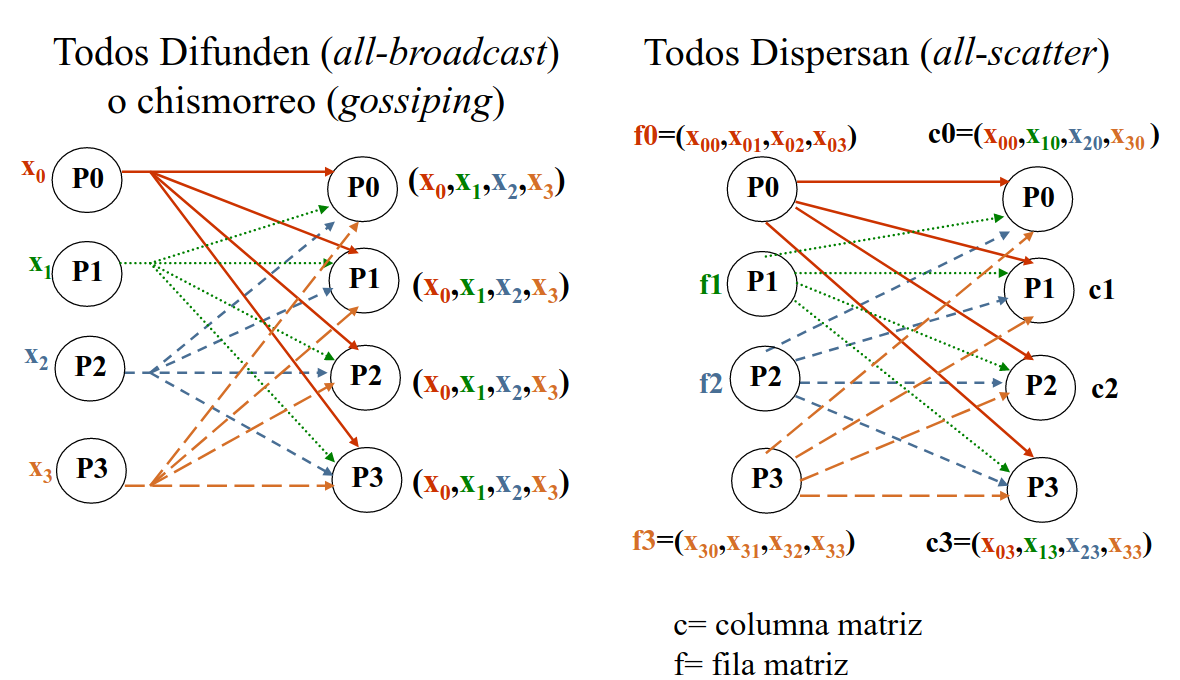
\includegraphics[scale=0.3]{todos_a_todos.png}
\caption{Comunicación todos a todos.}
\end{figure}

\subparagraph{Comunicaciones colectivas compuestas}

Las comunicaciones anteriores se pueden combinar dando lugar a nuevos servicios:

\begin{itemize}
	\item \textbf{Todos combinan o reducción y extensión}. Se aplica una reducción a todos los procesos, ya sea difundiéndola una vez obtenida (reducción y extensión) o bien realizándola en todos los procesos (todos combinan).
	\begin{figure}[H]
		\centering
		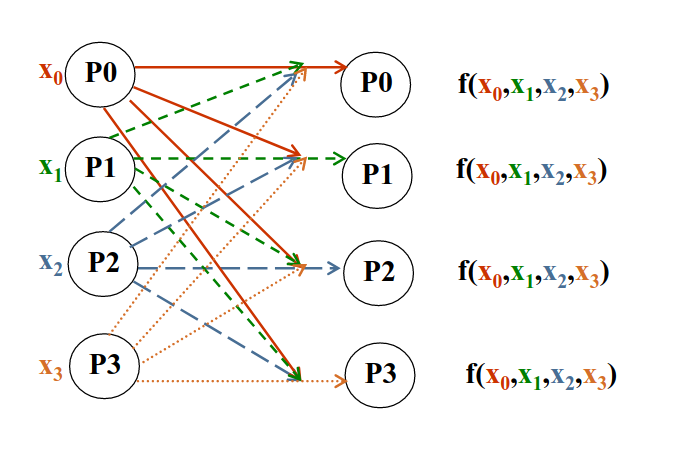
\includegraphics[scale=0.3]{todos_combinan.png}
		\caption{Todos combinan.}
	\end{figure}
	\item \textbf{Barrera}. Es un punto de sincronización que todos los procesos de un grupo deben alcanzar para poder continuar su ejecución. Se puede implementar mediante cerrojos o a nivel software.
	\item \textbf{Recorrido (\textit{scan})}. Todos los procesos envían un mensaje, recibiendo cada uno el resultado de reducir un conjunto de esos mensajes.
	\begin{figure}[H]
		\centering
		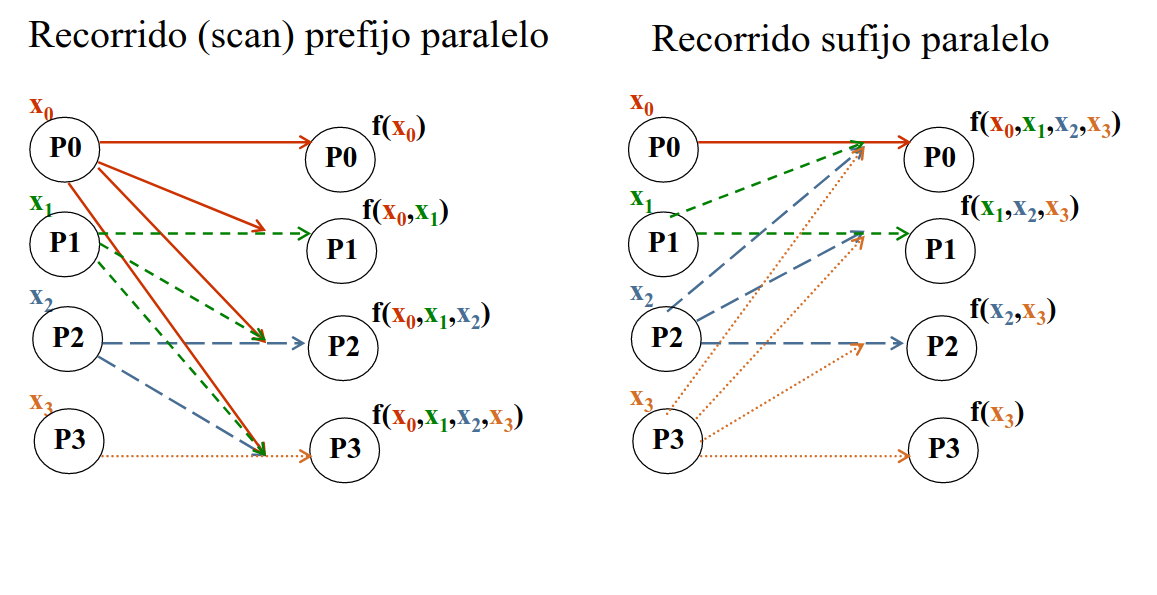
\includegraphics[scale=0.3]{scan.png}
		\caption{Recorrido (\textit{scan}).}
	\end{figure}
\end{itemize}
	
\subsubsection{Estilos de programación}

\paragraph{Paso de mensajes}

Disponemos de dos funciones principales:
\begin{itemize}
	\item \textbf{send(destino,datos)}. Envía datos.
	\item \textbf{receive(fuente,datos)}. Recibe datos.
\end{itemize}

Por lo general podemos encontrar transmisiones \emph{síncronas} (cuando ejecutamos un \emph{send}, el proceso se bloquea hasta que el destino recibe el dato y viceversa con \emph{receive}) o \emph{asíncronas} (\emph{send} no bloquea, por lo que suele hacerlo \emph{receive}).

La interfaz más conocida de paso de mensajes es MPI.

\paragraph{Variables compartidas}

La comunicación entre procesos se realiza accedeiendo a variables compartidas, es decir, mediante accessos y escrituras en memoria. Las hebras de un proceso creadas por el sistema operativo pueden compartir inmediatamente variables globales, pero los procesos no (tienen diferentes espacios de direcciones). En este caso, hemos de utilizar llamadas al sistema específicas.\\

La exclusión mutua se puede implementar mediante cerrojos, semáforos, variables condicionales, monitores, etc.\\

La interfaz más utilizada es OpenMP. Hay lenguajes, como Java, que implementan este paradigma.

\paragraph{Paralelismo de datos}

En este estilo se aprovecha el paralelismo de datos inherente a aplicaciones en las que los datos se organizan en estructuras (vectores o matrices). El programador escribe un programa con construcciones que permiten aprovechar el paralelismo: construcciones para paralelizar bucles, para distribuir datos, etc. Por tanto, no ha de ocuparse de las sincronizaciones, ya que son implícitas.\\

El lenguaje con paralelismo de datos más conocido es C* (\textit{C star}). En cuanto a APIs, destaca \textit{Nvidia CUDA}.

\begin{figure}[H]
	\centering
	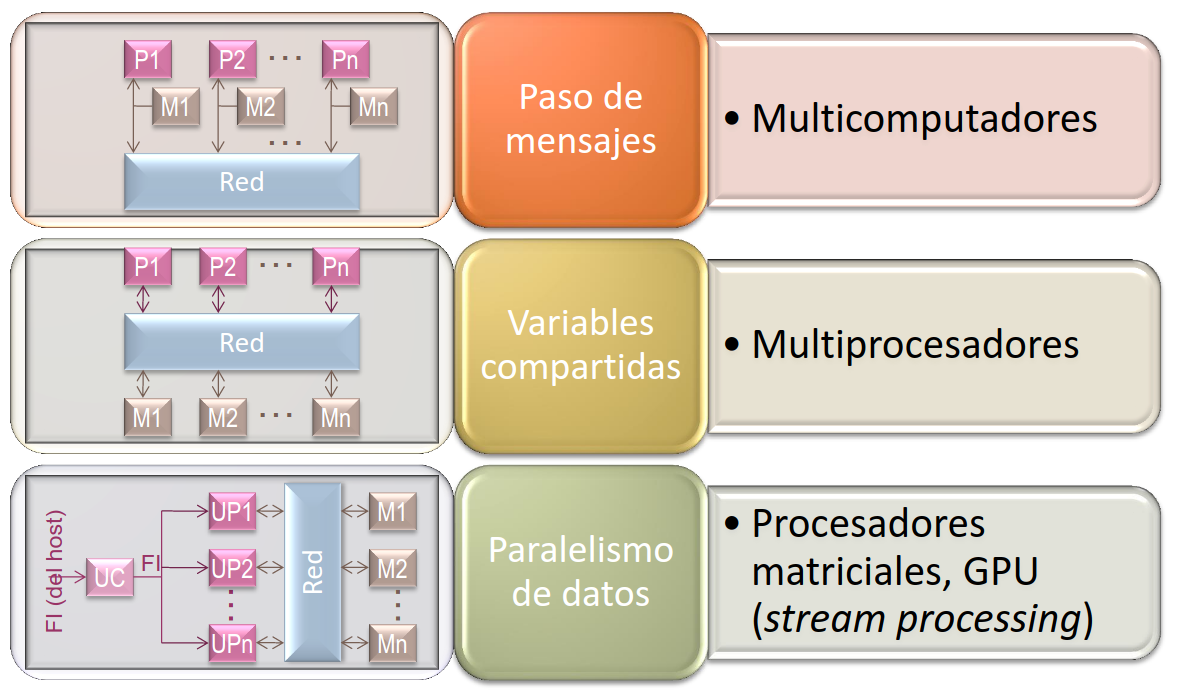
\includegraphics[scale=0.3]{estilos_programacion.png}
	\caption{Estilos de programación paralela.}
\end{figure}

\subsubsection{Estructuras de programas paralelos}

\paragraph{Dueño-esclavo (\textit{master-slave}) o granja de tareas (\textit{task-farming})}

Consta de un dueño y varios esclavos. El dueño se encarga de distribuir las tareas de un conjunto (granja) entre el grupo de esclavos y de ir recogiendo los resultados parciales que van calculando los esclavos. El dueño calcula el resultado final a partir de estos resultados parciales. Normalmente no hay comunicación entre los esclavos.\\

Se puede implemenmtar de forma mixta MPMD-SPMD con un programa para el dueño y otro para los esclavos o bien mediante SPMD con un sólo programa para ambos.

\begin{figure}[H]
	\centering
	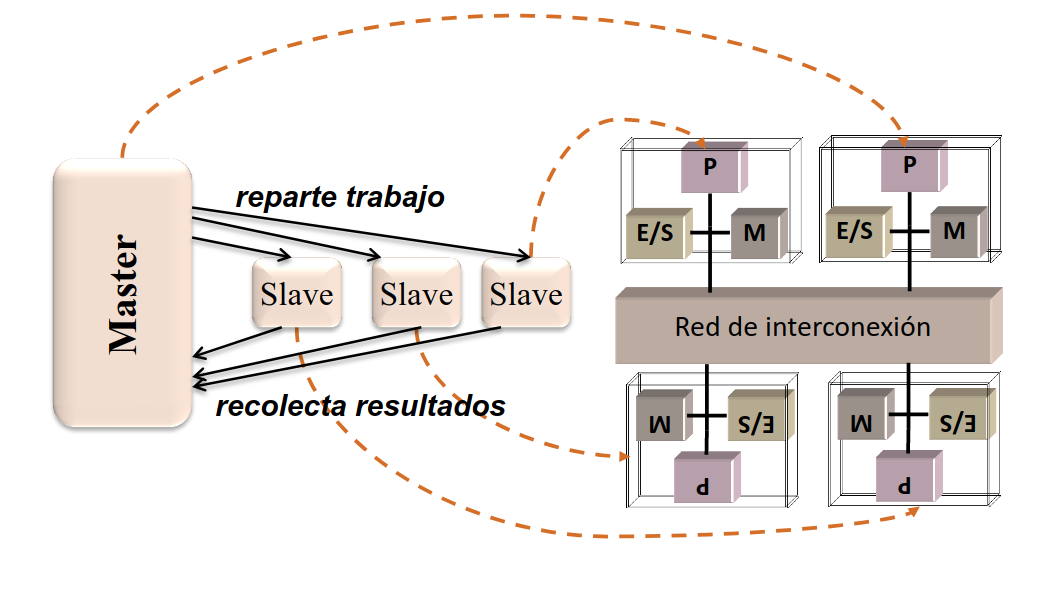
\includegraphics[scale=0.25]{maestro_esclavo.png}
	\caption{Dueño-esclavo.}
\end{figure}

\begin{figure}[H]
\centering
\begin{subfigure}[b]{0.3\textwidth}
\begin{minted}[linenos]{c++}
int main(){
/**Código dueño***/
}
--------------
int main(){
/**Código esclavo***/
}
\end{minted}
\caption{Dueño-esclavo como MPMD-SPMD}
\end{subfigure}
\hspace{5cm}
\begin{subfigure}[b]{0.3\textwidth}
\begin{minted}[linenos]{c++}
int main(){
 if(id_proc==id_duenio){
  /**Código dueño**/
 }
 else{
  /**Código esclavo**/
 }
}
\end{minted}
\caption{Dueño-esclavo como MPMD-SPMD}
\end{subfigure}
\caption{Diferentes implementaciones de dueño-esclavo.}
\end{figure}

\paragraph{Paralelismo de datos o descomposición de datos}

Esta alternativa se utiliza para obtener tareas paralelas en problemas en los que se opera con grandes estructuras de datos. La estructura de datos de entrada o la de salida (o ambas) se dividen en partes, de las que derivarán las tareas paralelas.

\begin{figure}[H]
	\centering
	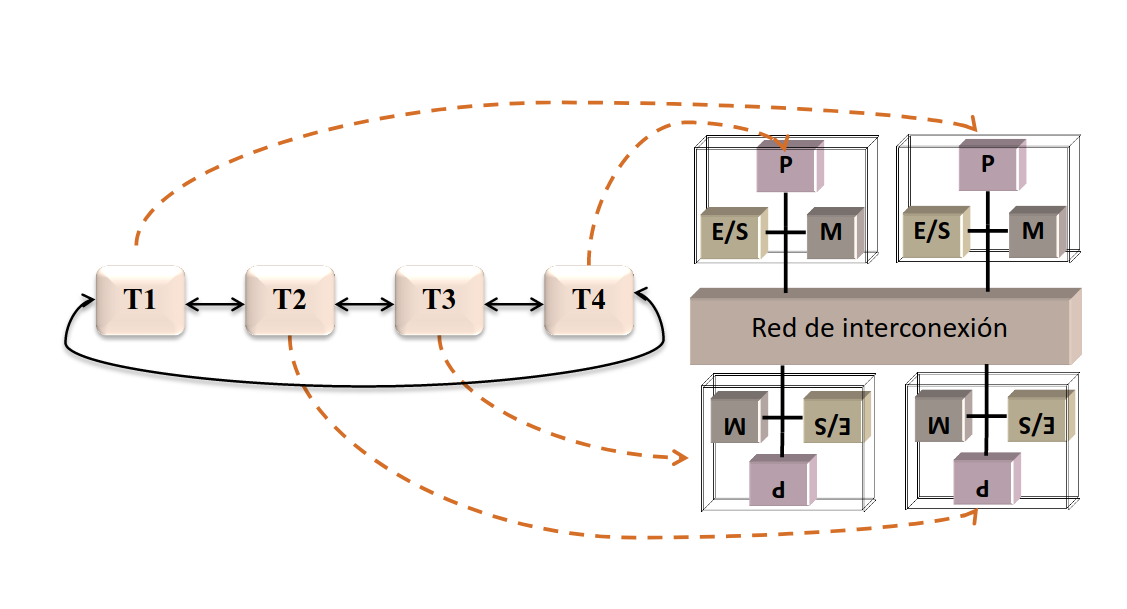
\includegraphics[scale=0.25]{descomposicion_datos.png}
	\caption{Descomposición de datos.}
\end{figure}

\paragraph{Divide y Vencerás}

Consiste en dividir un problema en dos o más subproblemas de forma que cada uno se pueda resolver de forma independiente y combinar los resultados para obtener el resultado final. Si los subproblemas son instancias más pequeñas que el original, podremos implementarlo mediante recursividad.

\begin{figure}[H]
\begin{subfigure}[b]{0.5\textwidth}
	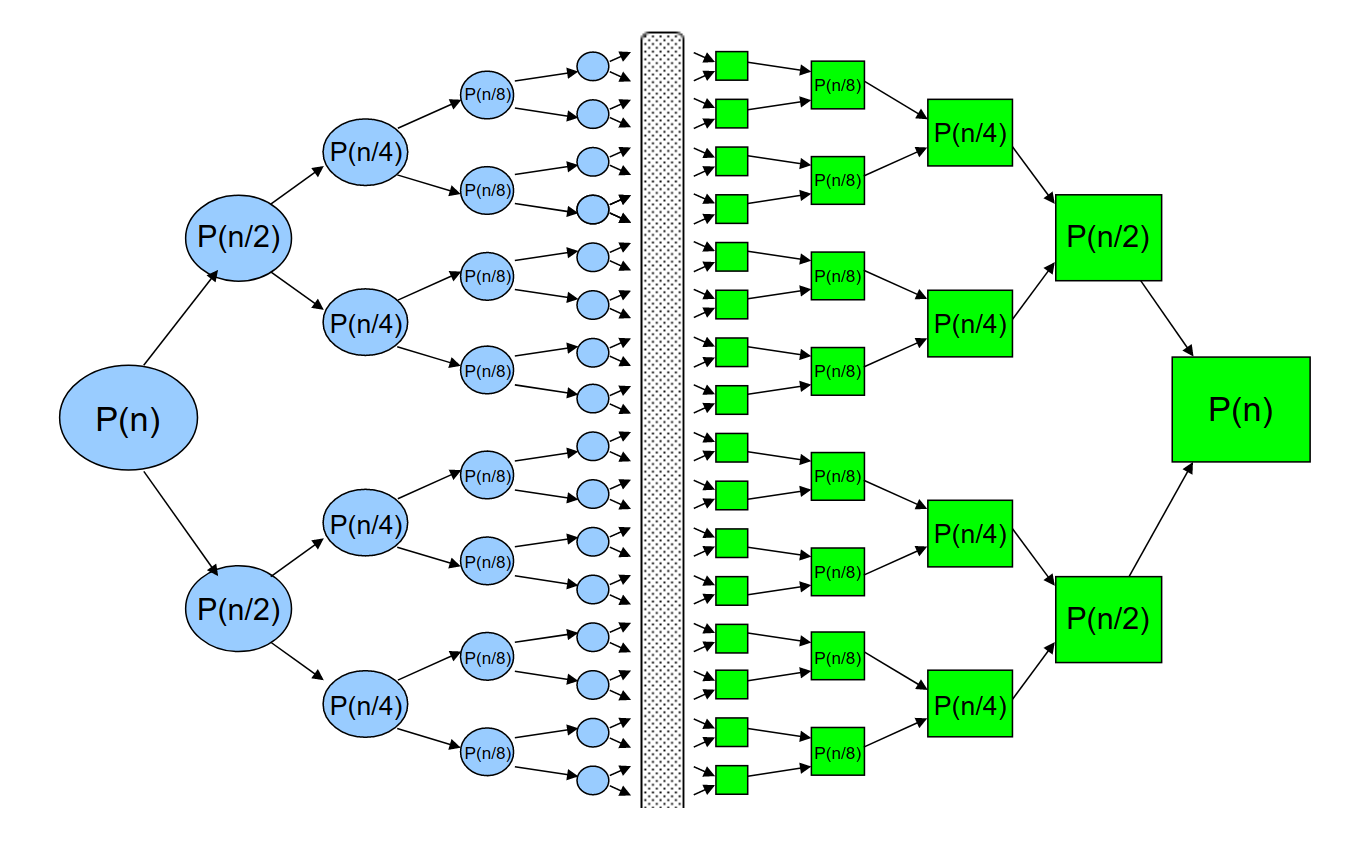
\includegraphics[width=\textwidth]{dyv.png}
\end{subfigure}
\quad
\begin{subfigure}[b]{0.5\textwidth}
	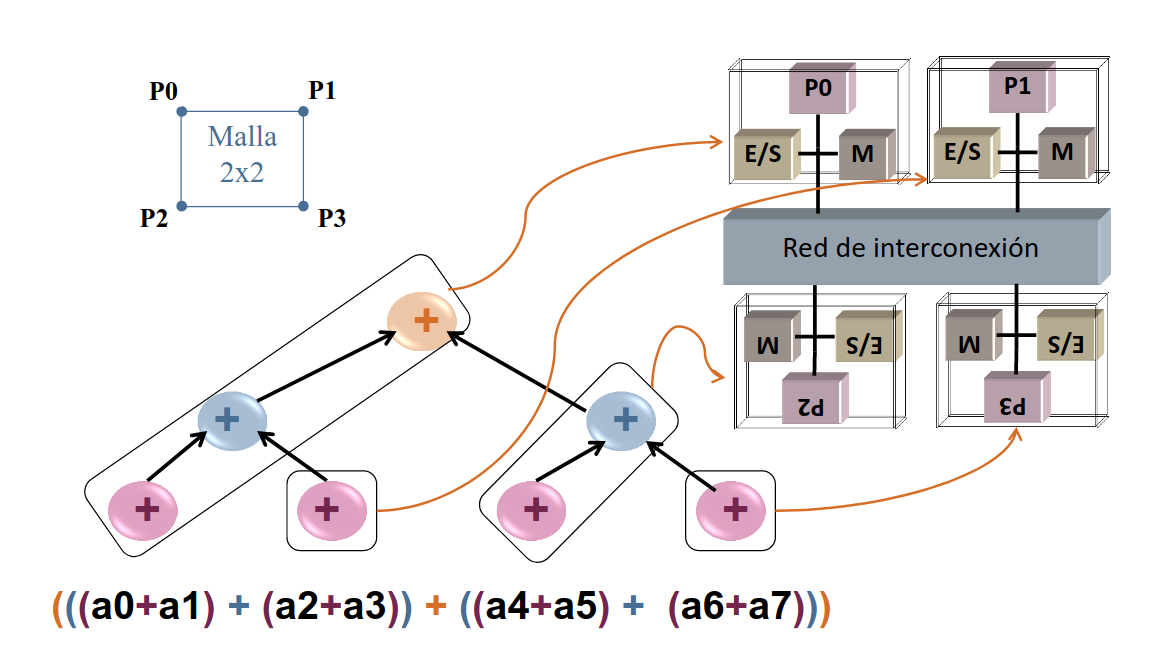
\includegraphics[width=\textwidth]{dyv_2.png}
\end{subfigure}
\caption{Divide y Vencerás.}
\end{figure}

\paragraph{Cliente-servidor}

Los clientes realizan peticiones a un servidor y éste les envía las respuestas.

\begin{figure}[H]
	\centering
	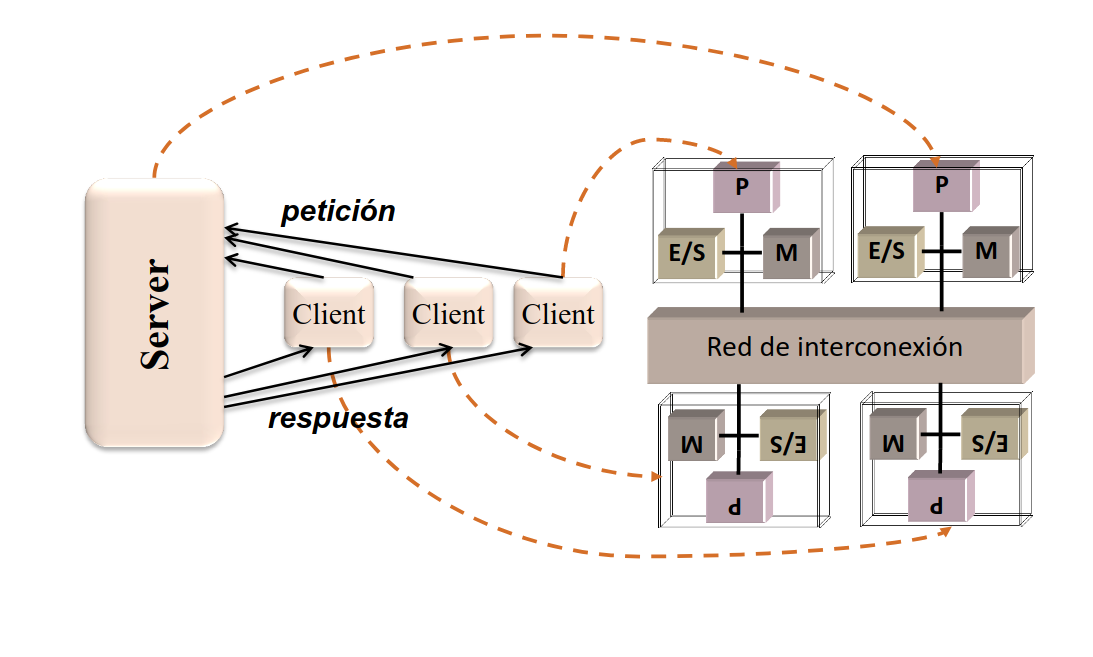
\includegraphics[scale=0.25]{cliente_servidor.png}
	\caption{Cliente-servidor.}
\end{figure}

\paragraph{Segmentada (\textit{pipeline}) o flujo de datos}

Aparece en probelmas en los que se aplican distintas funciones a un mismo flujo de datos (paralelismo de tareas). La estructura de procesos y de tareas es la de un cauce segmentado, por lo que cada proceso ejecuta distinto código (MPMD).

\begin{figure}[H]
	\centering
	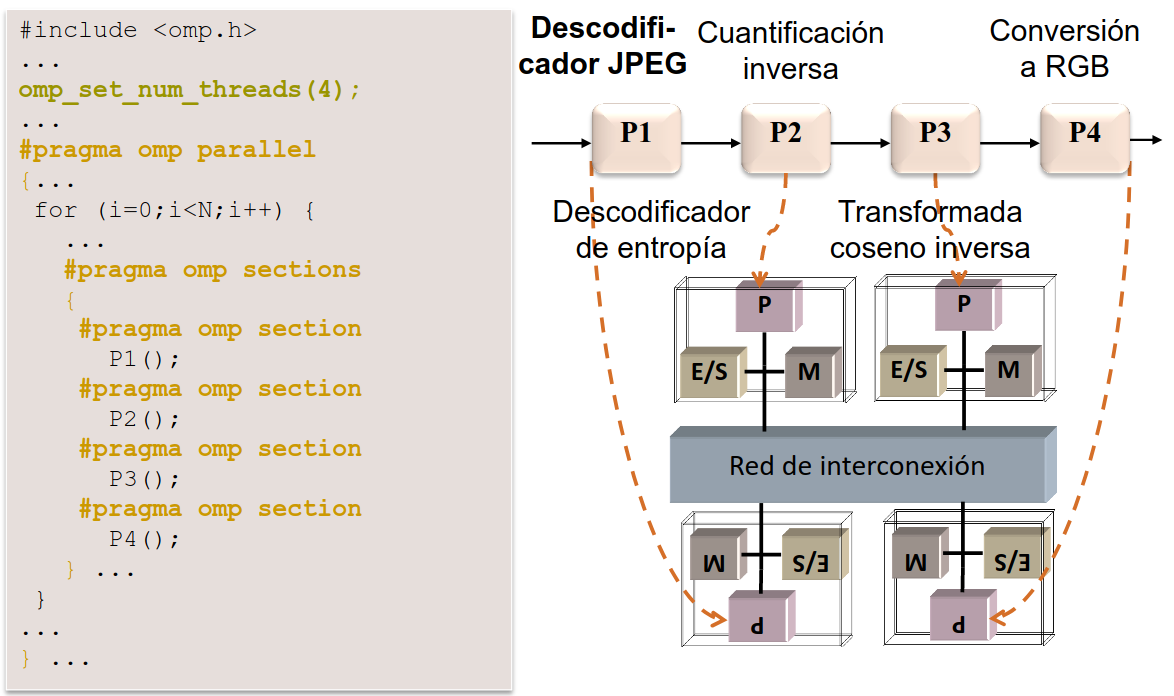
\includegraphics[scale=0.35]{segmentada.png}
	\caption{Segmentada (\textit{pipeline}). Decodificación JPEG.}
\end{figure}


\subsection{Proceso de paralelización}
Para obtener una versión paralela de una aplicación debemos seguir los siguientes pasos:
\begin{itemize}
	\item Descomponer la aplicación en tareas.
	\item Asignar tareas a procesos o hebras.
	\item Redactar código paralelo
	\item Evaluar prestaciones
\end{itemize}
\subsubsection{Descomposición de tareas}

En esta fase el programador busca unidades de trabajo independientes, es decir, que se podrán ejecutar en paralelo. Estas unidades, junto con los datos que utilizan, formarán las \textbf{tareas}. Podemos represetnar la estructura de las tareas (sus dependencias) meddiante un grafo dirigido en el que las aristas representen el flujo de datos y control y los vértices, las tareas.\\

El paralelismo se puede extraer en varios niveles de abstracción:
\begin{itemize}
	\item \textbf{Nivel de función}. Analizando las dependencias entre las funciones del código (paralelismo de tareas).
	\item \textbf{Nivel de bucle}. Analizando las iteraciones de los bucles dentro de una función (paralelismo de datos).
\end{itemize}

\begin{figure}[H]
	\centering
	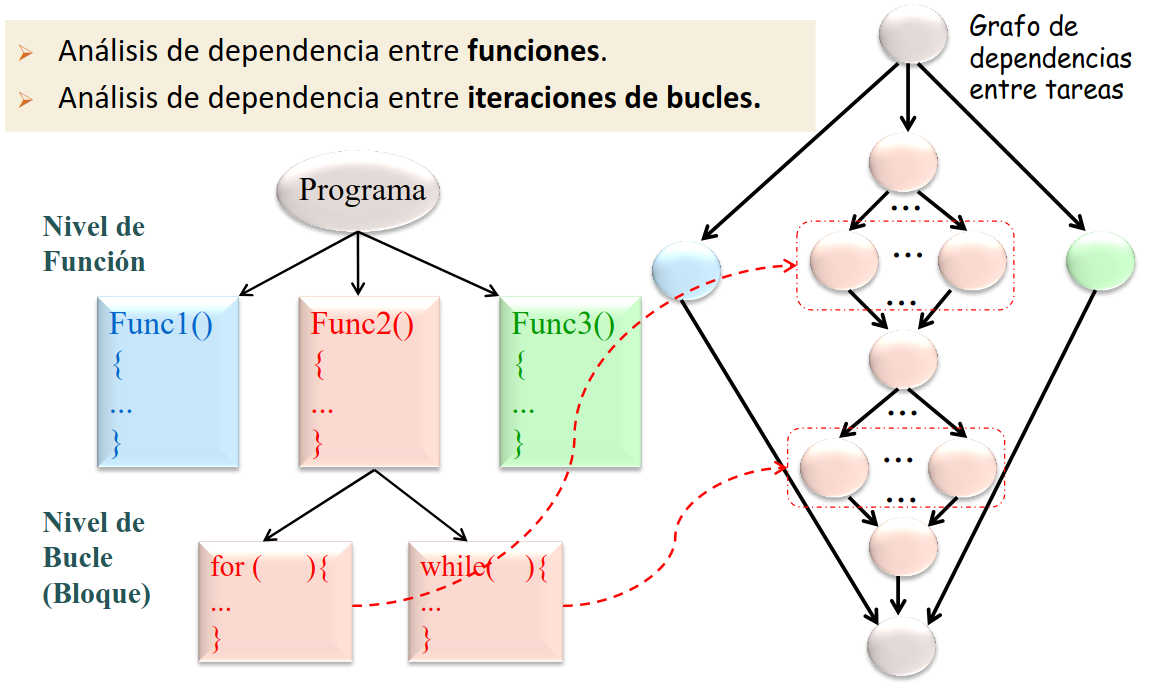
\includegraphics[scale=0.35]{grafo_dependencias_tareas.png}
	\caption{Segmentada (Grafo de dependencias entre tareas).}
\end{figure}

\subsubsection{Asignar tareas a procesos o hebras}

Esta etapa consiste en asignar las tareas del grafo de dependencias a procesos y a hebras. Por lo general, en una misma aplicación no resulta conveniente asignar más de un proceso o hebra por procesador, por lo que la asignación a procesos o hebras está ligada con la asignación a procesadores. Es más, se puede incluso realizar la asignación asociando los procesos (hebras) a procesadores concretos.\\

La posibilidad de utilizar procesos y/o hebras depende de varios factores:

\begin{itemize}
	\item La \textbf{arquitectura} en la que se va a ejecutar el programa. En un SMP (\textit{Symetric MultiProcessor}) y en procesadores multihebra es más eficiente usar hebras, mientras que en arquitecturas mixtas (como clústers de SMPs) es conveniente usar tanto hebras como procesos.
	\item El \textbf{Sistema Operativo} debe ser multihebra.
	\item La \textbf{herramienta de programación} debe permitir el uso de hebras.
\end{itemize}
Como regla básica, se tiende a asignar las iteraciones de un bucle (paralelismo de datos) a hebras y las funciones a procesos (paralelismo de tareas).\\

La asignación debe repartir la \emph{carga de trabajo} (tiempo de cálculo) optimizando la \emph{comunicación y sincronización}, de forma que todos los procesadores empiecen y terminen a la vez.\\

Las arquitecturas pueden ser heterogéneas u homogéneas. Si es \textbf{heterogénea}, consta de componentes con diferentes prestaciones, por lo que se deberá asignar más trabajo a nodos más rápidos. Una arquitectura \textbf{homogénea} puede ser muy uniforme o no. Si es \textbf{uniforme}, la comunicación de los procesadores con memoria (multiprocesadores) o entre sí (multicomputadores) supone el mismo tiempo sean cuales sean los nodos que intervienen.\\

Si la arquitectura es homogénea pero \textbf{no uniforme}, es más difícil asignar las tareas de forma que se minimice el tiempo de comunicación y sincronización (aristas en el grafo de tareas) y en general el tiempo de ejecución. \\

La asignación de tareas a procesadores (procesos, hebras) se puede realizar de forma \textbf{estática}, es decir, en tiempo de compilación o al escribir el programa o de forma \textbf{dinámica} (en tiempo de ejecución).


\subsubsection{Escribir el código paralelo}

El código dependerá del estilo de programación utilizado (variables compartidas, paso de mensajes, paralelismo de datos), del modo de programación (SPMD, MPMD, mixto,...), del punto de partida, etc.\\

En el programa habrá que añadir olas funciones, directivas o construcciones del lenguaje que hagan falta para:

\begin{itemize}
	\item Crear y terminar procesos.
	\item Localizar paralelismo.
	\item Asignar la carga de trabajo.
	\item Comunicar y sincronizar los diferentes procesos.
\end{itemize}
\subsubsection{Evaluación de prestaciones}

Una vez redactado el programa paralelo, se evaluarían sus prestaciones. Si no son las requeridas, se debe volver a etapas anteriores del proceso de implementación. Si volvemos a la etapa de escritura, podemos elegir otra herramienta de programación, ya que no todas ofrecen las mismas prestaciones.


\subsection{Prestaciones en computadores paralelos}

En computadores paralelos se utilizan principalmente las siguientes medidas de prestaciones:

\begin{itemize}
	\item \textbf{Tiempo de ejecución (respuesta)}. Es el tiempo que supone la ejecución de una entrada en el sistema.
	\item \textbf{Productividad (\textit{throughput})}. Es el número de entradas (aplicaciones) que el computador es capaz de procesar por unidad de tiempo.
\end{itemize}

Hay sistemas orientados a la mejora de la productividad (asignan cada entrada a un nodo de cómputo diferente), a la mejora del tiempo de respuesta (dividiendo el trabajo entre procesos) y orientados a ambos propósitos, como los servidores de internet.\\

También se utilizan otras medidas adicionales de prestaciones:

\begin{itemize}
	\item\textbf{Funcionalidad}. Cargas de trabajo para las que está orientado el diseño de la arquitectura.
	\item \textbf{Alta disponibilidad}. Presencia de recursos y software en el sistema para reducir el tiempo de inactividad y la degradación de prestaciones ante un fallo o por mantenimiento.
	\item \textbf{RAS (\textit{Reliability, Availability, Serviceability})}. Comprende tres propiedades cruciales: fiabilidad (capacidad del sistema de producir siempre los mismos resultados para las mismas entradas), disponibilidad (grado en el que un sistema sufre degradaciuón de prestaciones o detiene su funcionamiento por fallos o mantenimientos y serviciabilidad (facilidad con la que un técnico de hardware puede realizar el mantenimiento).
	\item \textbf{Tolerancia a fallos}. Capacidad de un sistema de mantenerse en funcionamiento ante un fallo.
	\item \textbf{Expansibilidad}. Posibilidad de expandir el sistema modularmente.
	\item \textbf{Escalabilidad}. Evolución del incremento (ganancia) en prestaciones que se consigue en el sistema conforme se añaden recursos (principalmente procesadorees). Pretende medir el nivel de aprovechamiento efectivo de los recursos.
	\item \textbf{Consumo de potencia}. Afecta a los costos de mantenimiento.
\end{itemize}

También se suele hablar de \textbf{eficiencia}, con la que se evalúa en qué medida las prestaciones que ofrece un sistema para sus entradas se acerca a las prestaciones máximas que idealmente debería ofrecer dados los recursos de los que dispone. Es decir, se emplea para evaluar en qué medida se utilizan los recursos del sistema.


\subsubsection{Ganancia en prestaciones. Escalabilidad}

Se emplea la ganancia en velocidad para estudiar en qué medida se incrementan las prestaciones al ejecutar una aplicación en paralelo en un sistema con múltiples procesadores frente a su ejecución en un sistema uniprocesador.
\begin{equation}
	S(p)=\frac{Prestaciones(p)}{Prestaciones(1)}
\end{equation}

Es decir, dividiendo las prestaciones conseguidas con un sistema multiprocesador entre las prestaciones obtenidas con la versión secuencial. Utilizando el tiempo de respuesta para evaluar prestaciones, quedaría:
\begin{equation}
S(p)=\frac{T_{secuencial}}{T_{paralelo}(p)}
\end{equation}
siendo $T_{paralelo}(p)=T_{computo}(p)+T_{overhead}(p)$\\
$T_{secuencial}$ debe ser el tiempo del mejor programa secuencial para la aplicación. En la penalización (\textit{overhead}) influyen factores como:
\begin{itemize}
	\item Tiempo de comunicación/sincronización entre procesos.
	\item Tiempo para crear/terminar procesos.
	\item Tiempo de ejecución de operaciones añadidas a la versión paralela no presentes en la secuencial.
\end{itemize}


Tanto el tiempo de cálculo paralelo como la sobrecarga dependen del número de procesos, Cuanto mayor sea, mayor será el \textit{grado de paralelismo} aprovechado. El grado de paralelismo para un programa es el número máximo de tareas independientes que se pueden ejecutar en paralelo. La sobrecarga depende del número de procesos involucrados.\\

La representación de la ganancia en función del número de procesadores nos permite evaluar la escalabilidad de una implementación paralela o una arquitectura.

\begin{figure}[H]
	\centering
	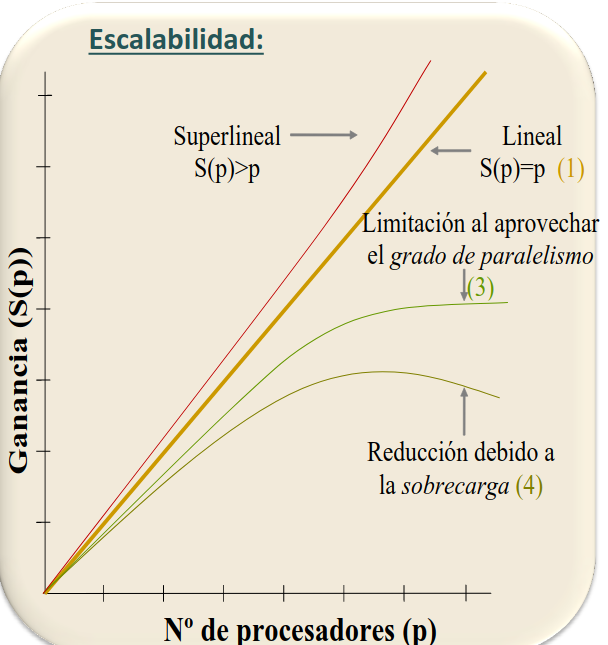
\includegraphics[scale=0.35]{escalabilidad.png}
	\caption{Segmentada (Ganancia frente a número de procesadores (escalabilidad).}
\end{figure}

Podemos ver que se dan varios casos:
\begin{enumerate}
	\item \textbf{Ganancia lineal}. El grado de paralelismo debe ser ilimitado, es decir, siempre se debe poder dividir el código entre los $p$ procesadores disponibles sea cual sea el valor de $p$. Además, el \textit{overhead} debe ser despreciable. $S_p=\frac{T_{secuencial}}{T_{paralelo}}=p$.
	\item \textbf{Ganancia superlineal} ($S_p>p$). Se debe a que al aumentar el número de procesadores aumentamos también el de otros recursos (caché, memoria principal, etc.) o bien a que la aplicación debe explorar varias posibilidades y termina cuando una es solución. 
	\item \textbf{Limitación al aprovechar el grado de paralelismo}. Se produce cuando hay código no paralelizable y la paralelización que se puede realizar no mejora las prestaciones.
	\item \textbf{Reducción debida a la sobrecarga}. Se produce cuando el incremento del número de procesadores no hace que el programa sea más rápido, pero sí que hace que el \textit{overhead} sea mayor.
\end{enumerate}


\paragraph{Ley de Amdahl}

Como vemos, la mejora en prestaciones está limitada por la fracción de código que no se puede paralelizar. Este razonamiento se formalizó por Amdahl mediante la siguiente ley:
\begin{equation}
	S(p)\leq \frac{p}{1+f(p-1)}
\end{equation}
donde:
\begin{itemize}
	\item $S$: incremento en velocidad que se consigue al aplicar una mejora.
	\item $p$: incremento en velocidad máximo que se puede conseguir si se usa siempre la mejora (número de procesadores).
	\item $f$: fracción de tiempo en la que no se utiliza la mejora (fracción de tiempo no paralelizable).
\end{itemize}

La ley de Amdahl nos dice que la escalabilidad está limitada por la fracción de tiempo no paralelizable. Sin embargo, en muchas aplicaciones podemos disminuirla aumentando el tamaño del problema, lo que conduce a un aumento de la ganancia.

\paragraph{Ganancia escalable. Ley de Gustafson}

Los objetivos al paralelizar una aplicación pueden ser:
\begin{itemize}
	\item Disminuir el tiempo de ejecución hasta que sea razonable.
	\item Aumentar el tamaño del problema a resolver, lo que nos puede llevar a mejoras como el aumento de la precisión.
\end{itemize}

Cuando llegamos a un nivel aceptable de tiempo de ejecución paralelo, el siguiente objetivo puede ser aumentar el tamaño del problema para poder mejorar otros aspectos de las prestaciones de la aplicación. Si consideramos el tiempo de \textit{overhead} insignificante, podemos mantener constante el tiempo de ejecución paralelo $T_p$ variando el número de procesadores $p$ y el tamaño $n$ de forma que $n=\Bbbk p$ con $\Bbbk \in \mathbb{R}$. Bajo estas condiciones, la ganancia en prestaciones sería:

\begin{equation}
S(p)=\frac{T_{secuencial}(n)}{T_{paralelo}}=\frac{f \cdot T_{paralelo} + p(1-f) \cdot T_{paralelo}}{T_{paralelo}}= p(1-f) + f
\end{equation}
donde $f$ representa la fracción de tiempo de la ejecución del programa paralelo que supone la ejecución de la parte no paralelizable. Cuanto mayor sea $1-f$, mayor será la escalabilidad.\\

Mientras que la Ley de Amdahl asume que el $T_{secuencial}$ (o tamaño de problema) es constante, Gustafson mantiene que lo constante es el $T_{paralelo}$. Ambos consideran despreciable el \textit{overhead}.

\paragraph{Eficiencia}

La eficiencia permite evaluar en qué medida las prestaciones ofrecidas por un sistema para un programa paralelo se acercan a las prestaciones máximas que idealmente debería ofrecer.

\begin{equation}
	E(p,n)=\frac{Prestaciones (p,n)}{Prestaciones (1,n)}=\frac{S(p,n)}{p}
\end{equation}
donde:
\begin{itemize}
	\item $p$ representa el número de recursos (procesadores).
	\item $n$ representa el tamaño del problema.
\end{itemize}


\newpage

\section{Tema 3}

\subsection{Arquitecturas TLP}

\subsubsection{Clasificación de arquitecturas con TLP explícito y una instancia de SO}

\begin{itemize}
	\item Los \textbf{multiprocesadores} ejecutan varios threads en paralelo en un computador (cada thread en un core distinto). 
	\item Los multiprocesadores en un chip (CMP) o \textbf{multicore} ejecutan varios threads en paralelo en un chip de procesamiento multicore (cada thread en un core distinto).
	\item Los \textbf{core multithread} son cores que modifican su arquitectura ILP para ejecutar threads concurrentemente (en paralelo)
\end{itemize}

\subsubsection{Multiprocesadores}
Ejecutan varios threads en paralelo en un computador (cada thread en un core distinto). 
\begin{figure}[H]
\centering
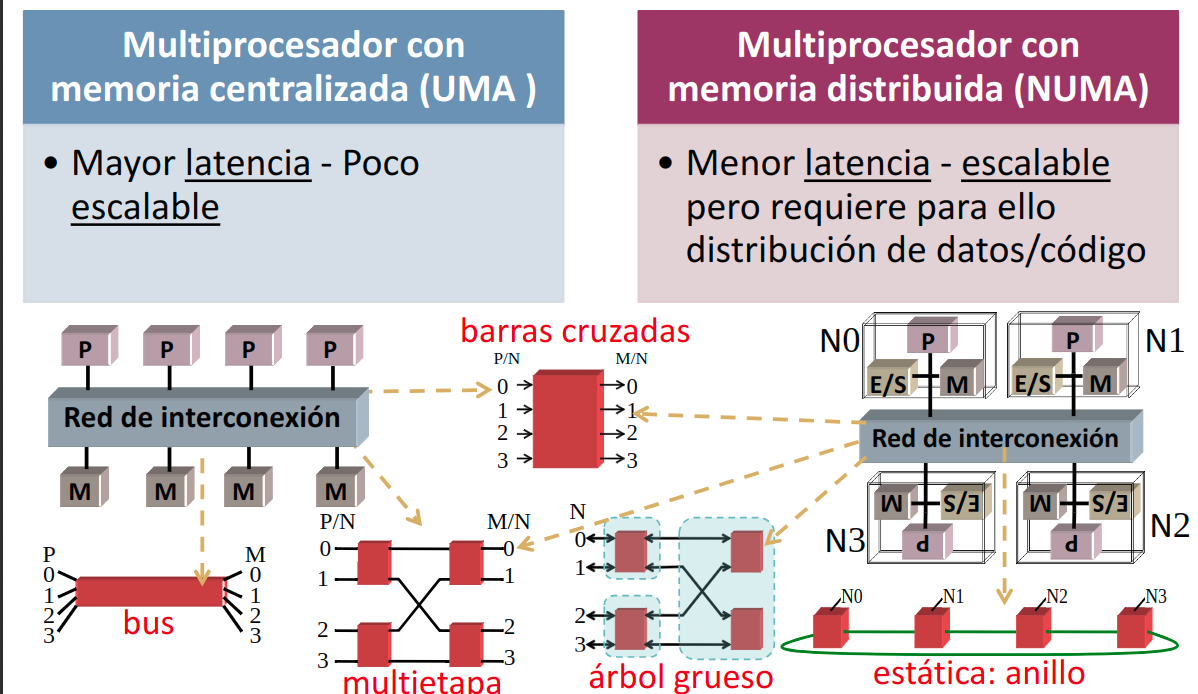
\includegraphics[scale=0.3]{uma_vs_numa.png}
\caption{Tipos de multiprocesadores según sistema de memoria.}
\end{figure}

\begin{figure}[H]
\centering
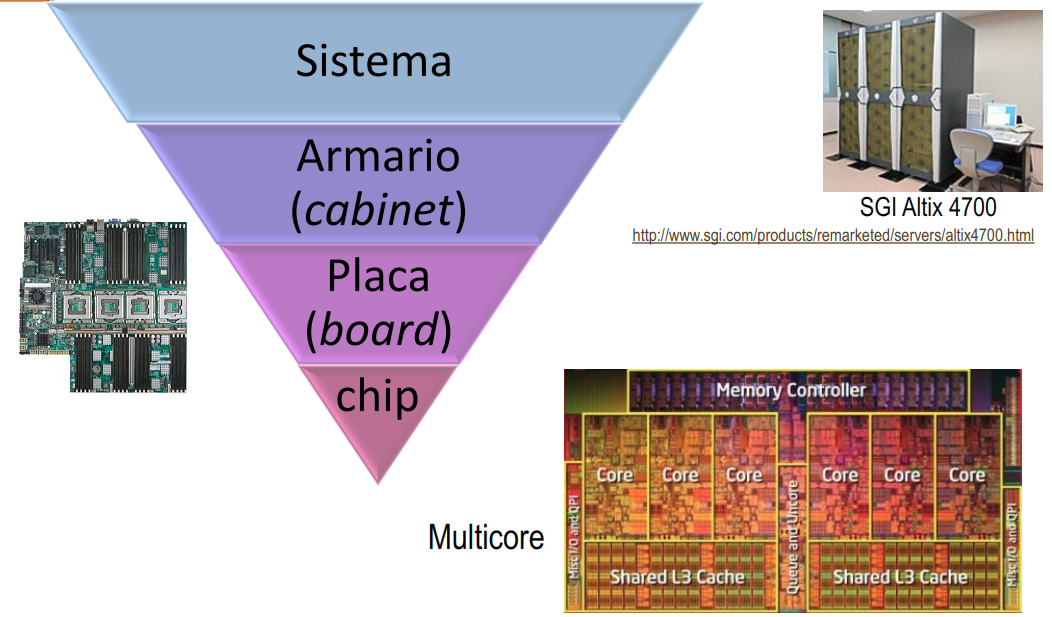
\includegraphics[scale=0.3]{uma_vs_numa_pack.png}
\caption{Tipos de multiprocesadores según empaquetamiento.}
\end{figure}

\begin{figure}[H]
\centering
\begin{subfigure}{0.3\textwidth}
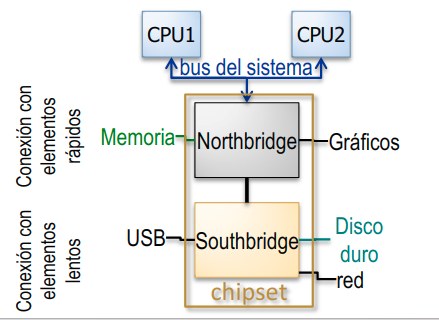
\includegraphics[width=\textwidth]{arq_uma.png}
\caption{UMA}
\end{subfigure}
\quad
\begin{subfigure}{0.3\textwidth}
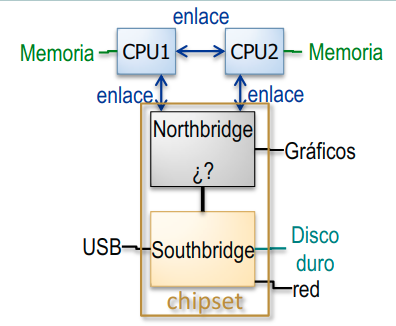
\includegraphics[width=\textwidth]{arq_numa.png}
\caption{NUMA}
\end{subfigure}
\vspace{1cm}
\begin{tabular}{|m{3cm}|m{5cm}|m{5cm}|}
\hline
&\textbf{UMA} & \textbf{NUMA} \\
 \hline
Controlador de memoria & Chipset (\textit{Northbridge)} & Chip del procesador \\
\hline
Red & Bus (compartido) & Enlaces (conexiones punto a punto) y conmutadores (en el chip del procesador).\\
\hline
\end{tabular}
\caption{Diferencias entre UMA y NUMA.}
\end{figure}

\begin{figure}[H]
\centering
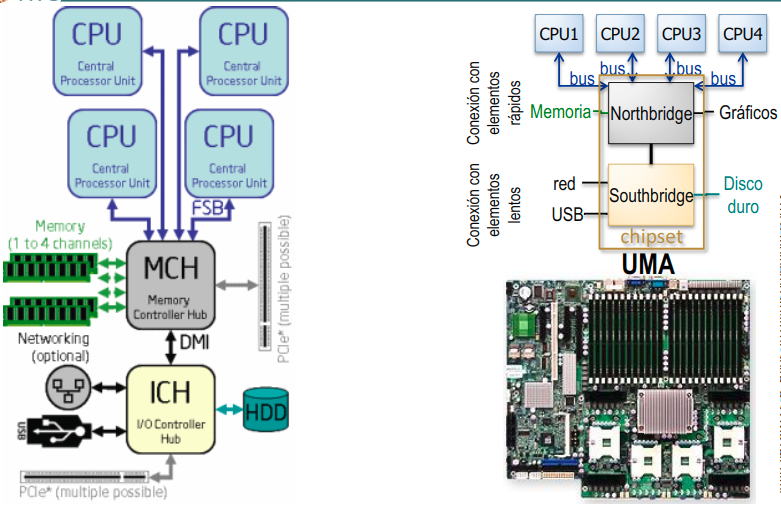
\includegraphics[scale=0.5]{placa_uma.png}
\caption{Placa base y CPU UMA.}
\end{figure}

\begin{figure}[H]
\centering
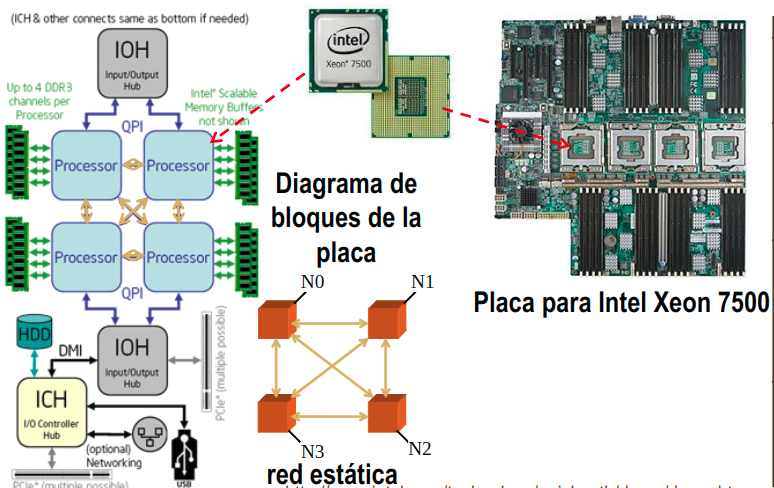
\includegraphics[scale=0.65]{placa_numa.png}
\caption{Placa base y CPU NUMA.}
\end{figure}


\subsubsection{Multicores}

Ejecutan varios threads en paralelo en un chip de procesamiento multicore (cada thread en un core distinto).

\begin{figure}[H]
\centering
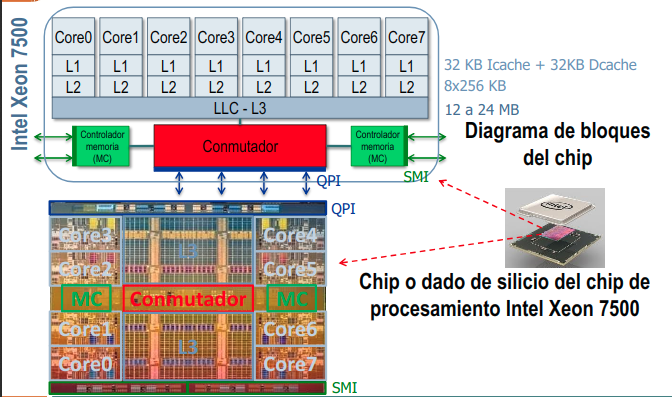
\includegraphics[scale=0.65]{cmp.png}
\caption{Ejemplo de multicore.}
\end{figure}

\begin{figure}[H]
\centering
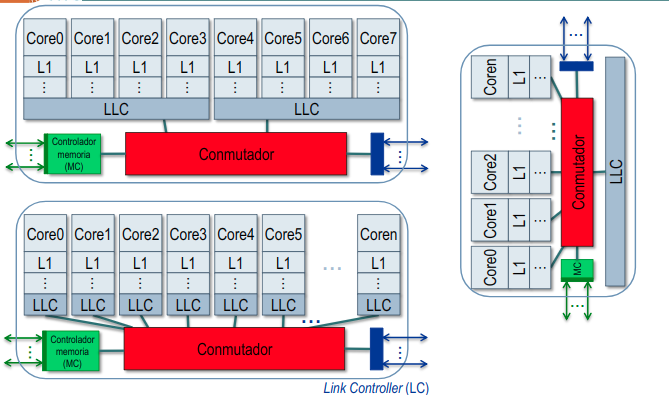
\includegraphics[scale=0.65]{cmp_arq.png}
\caption{Posibles arquitecturas de multicore.}
\end{figure}


\subsubsection{Cores multithread}

Modifican su arquitectura ILP (segmentada, escalar o VLIW) para ejecutar threads concurrentemente o en paralelo.

Las operaciones tienen varias estapas:
\begin{enumerate}
	\item Captación (\textbf{I}nstruction \textbf{F}etch).
	\item Decodificación y emisión a unidades funcionales (\textbf{I}nstruction \textbf{D}ecode).
	\item Ejecución (\textbf{Ex}ecution) y acceso a memoria (\textbf{Mem}ory).
	\item Almacenamiento de resultados (\textbf{W}rite-\textbf{B}ack).
\end{enumerate}

\begin{figure}[H]
\centering
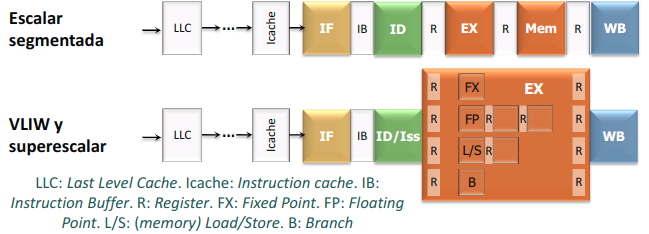
\includegraphics[scale=0.5]{tipos_ilp.png}
\caption{Tipos de arquitecturas ILP.}
\end{figure}

\begin{itemize}
	\item Los procesadores \textbf{segmentados} ejecutan instrucciones concurrentemente segmentando el uso de sus componentes.
	\item Los procesadores VLIW (\textit{Very Large Instruction Word} y los superescalares ejecutan las instrucciones concurrentemente (segmentación) y en paralelo (tienen múltiples unidades funcionales).
		\begin{itemize}
			\item VLIW
				\begin{itemize}
					\item Las instrucciones que se ejecutan en paralelo se captan juntas, formando la VLIW.
					\item El paralelismo (de instrucciones) es extraído mediante software.
				\end{itemize}
				\item Superescalares. El paralelismo de instrucciones es extraído mediante hardware específico.
		\end{itemize}
\end{itemize}

Los cores multithread se pueden clasificar en dos grandes grupos:

\begin{itemize}
	\item \textit{Temporal Multithreading} (\textbf{TMT}). 
	\begin{itemize}
		\item 	Ejecutan varios threads concurrentemente en el mismo core.
		\item La conmutación entre threads es gestionada por el hardware.
		\item Emite instrucciones de un único thread en un ciclo.
	\end{itemize}
	\item \textit{Simultaneus Multithreading} (\textbf{SMT}), multihilo simultáneo o \textit{horizontal multithread}.
		\begin{itemize}
			\item Ejecutan en un core superescalar varios threads en paralelo.
			\item Pueden emitir instrucciones de varios threads en un ciclo.
		\end{itemize}
\end{itemize}

A su vez, los cores TMT se pueden dividir en:

\begin{itemize}
	\item \textit{Fine-grain multithreading} (\textbf{FGMT}) o \textit{interleaved multithreading}.
	 La conmutación entre threads la decide el hardware en cada ciclo (coste 0). Utiliza algoritmos de planificación, como \textit{Round-Robin}.
	 \item \textbf{Coarse-grain mutithreading} (\textbf{CGMT}) o \textit{blocked multithreading}. La conmutación entre threads la decide el hardware (coste 0) en varios ciclos. Pueden ser en intervalos de tiempo prefijados o bien por eventos de cierta latencia.
\end{itemize}

Por último, los cores con CGMT y conmutación por eventos se clasifican en:

\begin{itemize}
	\item \textbf{Estática}. La conmutación puede ser explícita (instrucciones añadidas al repertorio) o implícita (usando instrucciones existentes). Su principal ventaja es que el coste del cambio de contexto es bajo (0/1 ciclo) y su inconveniente que se realizan cambios de contexto innecesarios.
	\item \textbf{Dinámica}. La conmutación se realiza por un fallo en la última caché, una interrupción, etc. Su principal ventaja es que reduce los cambios de contexto innecesarios pero aúin así se añade sobrecarga al realizar cambios de contexto.
\end{itemize}

\begin{figure}[H]
\centering
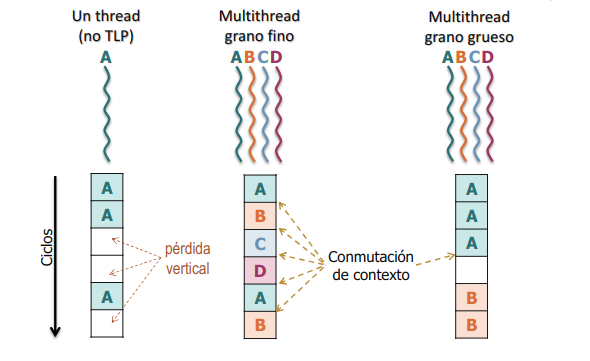
\includegraphics[scale=0.5]{alt_core_escalar_segmentado.png}
\caption{Alternativas en un core escalar segmentado (se emite una instrucción por ciclo).}
\end{figure}

\begin{figure}[H]
\centering
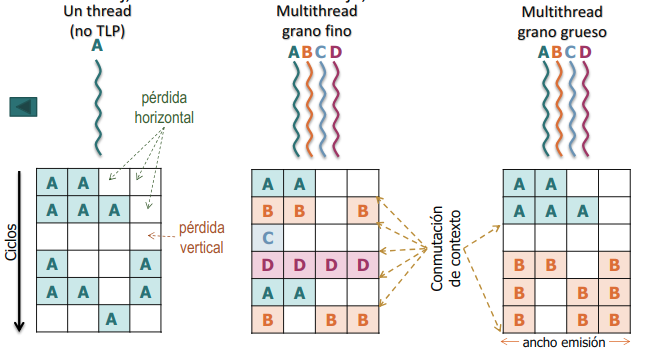
\includegraphics[scale=0.5]{alt_superescalar.png}
\caption{Alternativas en un core superescalar o VLIW (se emiten varias instrucciones por ciclo pertenecientes a un único thread).}
\end{figure}

\begin{figure}[H]
\centering
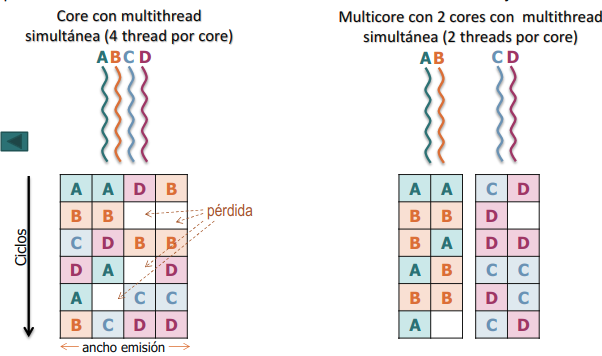
\includegraphics[scale=0.5]{alt_multicore.png}
\caption{Alternativas en multicores (se emiten instrucciones de distintos threads en cada ciclo).}
\end{figure}


\subsubsection{Hardware y arquitecturas TLP en un chip}

\begin{figure}[H]
\centering
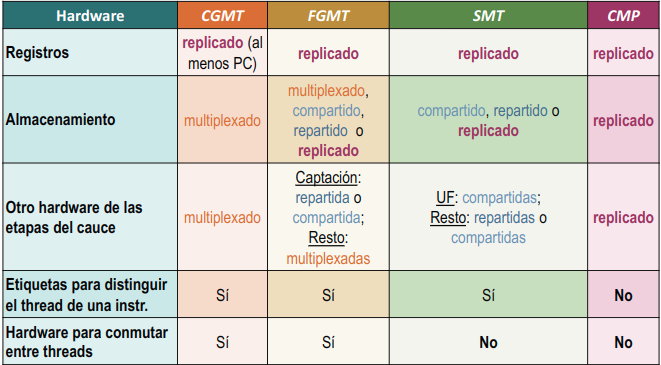
\includegraphics[scale=0.8]{arq_tlp.png}
\caption{Hardware y arquitecturas TLP en un chip.}
\end{figure}

\subsection{Coherencia del sistema de memoria}


\subsubsection{Sistema de memoria en multiprocesadores}

El uso de jerarquía de memoria con el fin de acercar la velocidad de acceso a memoria a la del procesador hace posible que pueda haber varias  copias de un mismo bloque en el sistema. Ésto puede ocurrir tanto en multiprocesadores como en uniprocesadores. El \emph{sistema de memoria} incluye las cachés de todos los nodos, memoria principal, controladores, buffers (escritura, combinación de escrituras, etc.) así como el medio de comunicación de estos componentes (red de interconexión).\\

La comunicación de datos entre procesadores es relizada por el sistema de memoria. Para que sea coherente, la lectura de una dirección debe devolver lo último que se ha escrito (desde el punto de vista de todos los componentes del sistema).

\begin{figure}[H]
\centering
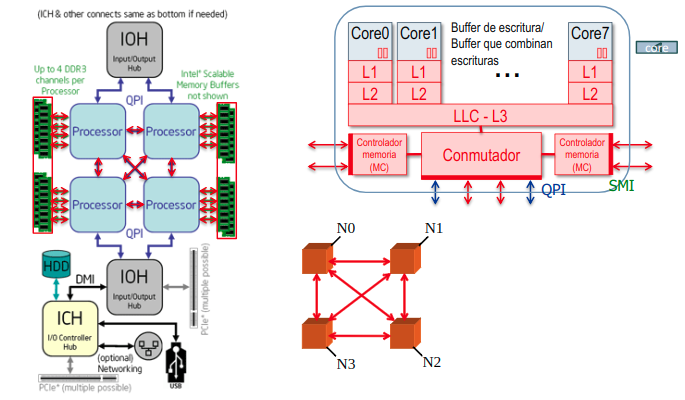
\includegraphics[scale=0.8]{sist_memoria.png}
\caption{Sistema de memoria.}
\end{figure}

\subsubsection{Concepto de coherencia en el sistema de memoria:  situaciones de incoherencia y requisitos para evitar problemas en estos casos}

Si en el sistema de memoria las copias de una dirección no tienen el mismo contenido, tendremos una \textbf{incoherencia en el sistema de memoria}. En sistemas con una sola caché se puede dar incoherencia entre la caché y la memoria principal. En sistemas con múltiples cachés la incoherencia se puede dar además entre las distintas cachés.

\begin{figure}[H]
\centering
\includegraphics[scale=0.8]{faltas_coherencia.png}
\caption{Tipos de estructuras de datos y faltas de coherencia.}
\end{figure}

\begin{figure}[H]
\centering
\includegraphics[scale=0.8]{ej_incoherencia.png}
\caption{Ejemplo de incoherencia.}
\end{figure}

\paragraph{Métodos de actualización de MP implementados en cachés.}

\begin{itemize}
	\item \textbf{Escritura inmediata} (\textit{write-through}). Cada vez que un procesador escribe en su caché escribe también en MP. Por tanto, cada escritura supone el uso de la red. No evita la incoherencias entre cachés.
	\item \textbf{Posescritura} (\textit{write-back}). La escritura se realiza cuando el bloque que contiene la dirección modificada se elimina de la caché para alojar un nuevo bloque. Con la posescritura se posibilitan incoherencias de caché y MP.
\end{itemize}

La falta de coherencia entre cachés y los problemas de incoherencias se pueden solventar mediante hardware específico de coherencia. Existen alternativas para abordar las incoherencias entre caché y MP si el sistema no tiene hardware específico de mantenimiento de coherencia. Por ejemplo, se puede evitar la falta de coherencia declarando las zonas de memoria implicadas en la comunicación como \emph{no cacheables} o bien con escritura inmediata. \\

Como ya hemos visto, en sistemas con múltiples cachés puede haber faltas de coherencia entre cachés, tanto con escritura inmediata como con posescritura. Los \textbf{protocolos de coherencia de caché} resuelven este problema haciendo que cada escritura sea visible a todos los procesadores, propagando de forma fiable un nuevo valor escrito en una dirección.

\paragraph{Alternativas para propagar una escritura en protocolos de coherencia de caché.}

\begin{itemize}
	\item \textbf{Escritura con actualización} (\textit{write-update}). Cada vez quee un procesador escribe en una dirección en su caché, se escribe el nuevo dato en las copias de esa dirección de las otras cachés.
	\item \textbf{Escritura con invalidación} (\textit{write-invalidate}). Antes de que un procesador modifique una dirección en su caché se invalidan las copias del bloque de la dirección en otras cachés. Cuando otro procesador quiera leer la información tendrá un fallo de caché, por lo que obtendrá el dato actualizado.
\end{itemize}

Hay que tener en cuenta que puedo ocurrir que la propagación de una escritura a todos los procesadores a través de la red de interconexión requiera un tiempo distinto para cada procesador. En ese caso, si se solaparan varias propagaciones, distintos procesadores podrían recibir y leer en distinto orden las escrituras, causando incoherencia.

\paragraph{Requisitos del sistema de memoria para evitar incoherencias}

\begin{itemize}
	\item La escritura en una dirección debe hacerse visible en un tiempo finito a los otros procesadores.
	\item Las escrituras en una misma dirección deben verse en el mismo orden por todos los procesadores. Es decir, las operaciones de escritura en la misma dirección se deben realizar en serie (una detrás de otra).
\end{itemize}


Las comunicaciones uno a muchos para actualizar o invalidar las copias del bloque que se modifica se pueden implementar en un bus, ya que permite la difusión de forma natural. En buses se utilizan \textbf{protocolos de espionaje (snoopy)}, que aprovechan que todos los componentes conectados al bus pueden ver (espiar) su contenido. El controlador de caché espía los parquetes en el bus y actúa en consecuencia (por ejemplo, invalidando o actualizando la copia que tienen de un bloque). \\

En redes en las que la difusión es costosa de implementar o en las que se requiere una mayor escalabilidad se usan \textbf{esquemas basados en directorios}. En ellos se envían paquetes únicamente a las cachés implicadas para reducir el tráfico. La información sobre las cachés implicadas en cada momento se almacena en un directorio asociado a la memoria principal.\\

Este directorio centralizado (monolítico), al igual que el bus, supone un cuello de botella. Podemos obtener mejores prestaciones si lo distribuimos entre los módulos de memoria principal. Es decir, el subdirectorio de cada módulo mantiene información de los bloques que conteien el módulo. Los diferentes subdirectorios procesan peticiones en paralelo.

\begin{figure}[H]
\centering
\includegraphics[scale=0.7]{directorio_mp.png}
\caption{Directorio de memoria principal.}
\end{figure}

\begin{figure}[H]
\centering
\includegraphics[scale=0.75]{tipos_directorios.png}
\caption{Alternativas para implementar el directorio.}
\end{figure}

El hecho de que las operaciones de acceso a memoria tengan que llegar al directorio para obtener información de un bloque (cachés implicadas) permite usar el directorio para establecer un orden entre accesos a una misma dirección (serializar) de forma que todos los procesadores vean este mismo orden. No obstante, en algunos sistemas se pueden necesitar paquetes de reconocimiento de actualizaciones o invalidaciones que confirmen que ha finalizado una escritura anterior e información de estado para el bloque en el directorio (si está pendiente de finalizar un acceso).\\

También se pueden encontrar esquemas de coherencia de caché organizados en \textbf{jerarquía} compuestos de protocolos de espionaje y directorios, según la red de cada nivel.

\begin{itemize}
	\item Protocolos de \textbf{espionaje} (\textit{snoopy}). Para buses y en general sistemas con difusión eficiente (pocos nodos o red que implementa difusión).
	\item Protocolos basados en \textbf{directorios}. Para redes sin difusión o escalables.
	\item Esquemas \textbf{jerárquicos}. Se usan para redes jerárquicas: jerarquía de buses, de redes escalables, redes escalables-buses, etc.
\end{itemize}
\captionof{figure}{Protocolos para mantener coherencia en el sistema de memoria.}


\subsubsection{Protocolo MSI de espionaje}

También se denomina protocolo de invalidación de tres estados. Utiliza posescritura y escritura con invalidación. \\

Un bloque puede tener tres estados:
\begin{itemize}
	\item \textbf{Modificado} (M). Es la única copia válida del bloque en todo el sistema. La caché debe proporcionar el bloque si al espiar el bus observa que algún componente la solicita e invalidarlo si algún nodo solicita una copia exclusiva para su modificación.
	\item \textbf{Compartido} (S). Todas las copias del bloque están actualizadas. La caché debe invalidar su copia si al espiar el bus observar que algún nodo solicita una copia exclusiva del bloque para su invalidación.
	\item \textbf{Inválido} (I). El bloque se ha invalidado o bien no se encuentra físicamente en caché.
\end{itemize}

Por su parte, un bloque puede ser:

\begin{itemize}
	\item \textbf{Válido}. Tiene una copia válida. Es decir, el controlador puede proporcionar el bloque en caso de solicitud.
	\item \textbf{Inválido}. La copia no es la última actualización, es decir, hay una caché que ha modificado el bloque (estado modificado).
\end{itemize}

Un nodo terminal puede generar las siguientes transferencias como consecuencia de acciones de lectura/escritura en la caché del procesador o bien como consecuencia de paquetes recibidos de otros nodos:

\begin{itemize}
	\item Petición de lectura de un bloque (\textbf{PtLec}). Un procesador lee de una dirección que no se encuentra en su caché (fallo de caché). El controlador inicia la transacción poneidno en el bus la dirección a la que desea acceder. El sistema de memoria proporcionará el bloque donde se encuentra la dirección solicitada.
	\item Petición de acceso exclusivo (\textbf{PtLecEx}). Se genera por la escritura de un procesador (PrEsc) en un bloque compartido o inválido. El controlador de caché genera el paquete que indicará la dirección en la que se desea escribir. El resto de cachés con copias válidas las invalidarán. También se invalidará el bloque en memoria si se encuentra en estado válido. El procesador puede solicitar una confirmación de este paquete.
	\item Petición de posescritura (\textbf{PtPEsc}). Se genera por el reemplazo de un bloque modificado debido a un fallo de caché (se sobreescribe el bloque con estado modificado). El procesador del nodo no conoce este hecho y no espera respuesta.
	\item Respuesta con bloque (\textbf{RpBloque}). La genera un nodo que observa en el bus una petición de un bloque que tiene en estado modificado solicitada por una petición de lectura (exclusiva o no).
\end{itemize}

\begin{figure}[H]
\centering
\includegraphics[scale=0.75]{msi.png}
\caption{Descripción de MSI.}
\end{figure}

\subsubsection{Protocolo MESI de espionaje}

También denominado protocolo de invalidación de cuatro estados. También utiliza posescritura y escritura con invalidación.\\

En el protocolo MSI, si un procesador escribía en un bloque de su caché tenía que generar una transferencia que invalidase copias en otras cachés, aunque no hubiera copias del bloque en cachés de otros procesadores. Este hecho degrada las prestaciones de aplicaciones secuenciales ejecutadas en multiprocesadores, ya que no comparten variables entre procesos. \\

Para solventar este problema se añade un nuevo estado: \emph{exclusivo}. Un bloque en estado exclusivo será válido sólo en la caché en la que se encuentra y en memoria. Si un bloque se encuentra en estado exclusivo en la caché de un nodo y el procesador del nodo escribe en el bloque, no se genera paquete para solicitar uso exclusivo e invalidar copias, ya que sabemos que ninguna otra caché tiene copia válida.\\

Los posibles estados de un bloque son:

\begin{itemize}
	\item \textbf{Modificado} (M). Es la única copia válida en todo el sistema.
	\item \textbf{Exclusivo} (E). Es la única caché en el sistema con una copia válida del bloque, el resto tienen una copia no válida. La memoria tiene también una copia actualizada del bloque. La caché debe invalidar su copia si observa que algún otro nodo solicita una copia exclusiva del bloque para su modificación.
	\item \textbf{Compartido}  (C). El bloque es válido, también en memoria y en al menos alguna otra caché. La caché debe invalidar su copia si observa que algún otro nodo solicita una copia exclusiva del bloque para su modificación.
	\item \textbf{Inválido} (I). El bloque no está físicamente en caché o bien está en estado no válido.
\end{itemize}

\begin{figure}[H]
\centering
\includegraphics[scale=0.75]{mesi.png}
\caption{Descripción de MESI. Quitando lo tachado se obtiene MSI.}
\end{figure}

\subsubsection{Protocolo MSI basado en directorios con o sin difusión}

\paragraph{MSI con directorios sin difusión}

Un bloque en caché puede tener tres estados distintos: \textbf{modificado} (M), \textbf{compartido} (C) o \textbf{inválido} (I).\\

Un bloque en MP puede ser \textbf{válido} o \textbf{inválido}.\\

Hay varios tipos de nodos: \textbf{solicitante} (S), origen (O), modificado (M), propietario (P) y compartidor (C).

Si un nodo \textbf{S} realiza una petición a un nodo \textbf{O}, la petición puede ser:

\begin{itemize}
	\item Lectura de bloque (\textbf{PtLec}).
	\item Lectura con acceso exclusivo (\textbf{PtLecEx}).
	\item Petición de acceso exclusivo sin lectura (\textbf{PtEx}).
	\item Posescritura (\textbf{PtPEsc}).
\end{itemize}

Los nodos \textbf{O} pueden reeviar a los nodos con copia (\textbf{P},\textbf{M} o \textbf{C}) varias peticiones: invalidación (\textbf{RvInv}) o lectura (\textbf{RvLec} o \textbf{RvLecEx}).\\

También pueden recibir respuestas:
\begin{itemize}
	\item Nodo \textbf{P} a \textbf{O}: respuesta con bloque (\textbf{RpBloque}) o respuesta con/sin bloque confirmando invalidación (\textbf{RpInv}, \textbf{RpBloqueInv}).
	\item Nodo \textbf{O} a \textbf{S}: respuesta con bloque (\textbf{RpBloque}), respuesta con o sin bloque confirmando fin de invalidación (\textbf{RpInv},\textbf{RpBloqueInv}).
\end{itemize}

\begin{figure}[H]
\centering
\includegraphics[scale=0.75]{msi_dir_nodif.png}
\caption{MSI con directorios sin difusión.}
\end{figure}

\paragraph{MSI con directorios con difusión}

Un bloque en caché puede tener tres estados distintos: \textbf{modificado} (M), \textbf{compartido} (C) o \textbf{inválido} (I).\\

Un bloque en MP puede ser \textbf{válido} o \textbf{inválido}.\\

Hay varios tipos de nodos: \textbf{solicitante} (S), origen (O), modificado (M), propietario (P) y compartidor (C).\\

Difusión de petición del nodo S a:
\begin{itemize}
	\item \textbf{O} y \textbf{P}: lectura de un bloque (\textbf{PtLec}), lectura con acceso exclusivo (\textbf{PtLecEx}), petición de acceso exclusivo sin lectura(\textbf{PtEx}).
	\item \textbf{O}: posescritura (\textbf{PtPEsc}).
\end{itemize}

Respuesta de:

\begin{itemize}
	\item Nodo \textbf{P} a \textbf{O}: respuesta con bloque (\textbf{RpBloque}) o respuesta con/sin bloque confirmando invalidación (\textbf{RpInv}, \textbf{RpBloqueInv}).
	\item Nodo \textbf{O} a \textbf{S}: respuesta con bloque (\textbf{RpBloque}), respuesta con o sin bloque confirmando fin de invalidación (\textbf{RpInv}
\end{itemize}

\begin{figure}[H]
\centering
\includegraphics[scale=0.75]{msi_dir_dif.png}
\caption{MSI con directorios con difusión.}
\end{figure}

\subsection{Consistencia del sistema de memoria}

\subsubsection{Concepto de consistencia de memoria}

Un \textbf{modelo de consistencia de memoria} especifica el orden el el cual las operaciones de aceso a memoria (lectura/escritura) deben \textit{parecer} haberse realizado.\\

La coherencia sólo abarca operaciones realizadas por múltiples componentes (procesos o procesadores) sobre una misma dirección.\\


\subsubsection{Consistencia secuencial}

En un sistema uniprocesador, este orden es el orden secuencial ejecutado por el programador, denominado \textbf{orden del programa}. Sin embargo, el hardware o el compilador pueden alterar el orden de las instrucciones para mejorar prestaciones, pero debe parecer que no se ha alterado para garantizar el modelo de consistencia al programador. En concreto, se debe garantizar que:

\begin{itemize}
	\item Cada lectura de una dirección proporcione el último valor escrito en esa ddirección (dependencia RAW).
	\item Si se escribe varias veces en una dirección se debe retornar el último valor escrito (dependencia WAW).
	\item Si se escribe en una dirección que ha sido previamente leída, no se debe obtener en la lectura previa el valor escrito posteriormente (dependencia WAR).
	\item No se puede escribir en una dirección si la escritura depende de una condición que no se cumple (dependencias de control).
\end{itemize}

El \textbf{modelo de consistencia secuencial (SC)} requiere que todas las operaciones de memoria parezcan ser ejecutadas una cada vez (ejecución \emph{atómica}) y que todas las operaciones de un único procesador o proceso parezcan ejecutarse en eel \emph{orden descrito} por el programa de entrada al procesador.\\

El modelo de consistencia secuencial es el que suele esperar el programador a alto nivel, ya que presenta el sistema de memoria como una memoria global conectada a todos los procesadores a través de un conmutador central.

\begin{figure}[H]
\centering
\includegraphics[scale=0.75]{modelo_sc.png}
\caption{Presentación del sistema a los programadores mediante el modelo SC.}
\end{figure}

\paragraph{Ejemplo} Supongamos que disponemos del siguiente código:
\begin{minted}[linenos]{c++}
P1{
	A=1;	//Escribir A
	K=1;	//Escribir K
}
/*******************/
P2{
	while(k==0){}	//Leer K
	var=A;	//Leer A
}
\end{minted}


\begin{figure}[H]
\centering
\includegraphics[scale=0.75]{ej_sc.png}
\caption{Ejemplo de ejecución con SC.}
\end{figure}

\subsubsection{Modelos de consistencia relajados}

Los modelos de memoria relajados difieren en cuanto a los requisitos para garantizar conssitencia secuencial (SC) relajan:
\begin{itemize}
	\item \textbf{Orden del programa}. Pueden permitir que en el código ejecutado en un procesador se relaje el orden entre dos accesos a distintas direcciones. Pueden permitir relajar distintos órdenes: $W \rightarrow W$,$W \rightarrow R$ , $R \rightarrow W$ o $R \rightarrow R$.
	\item \textbf{Atomicidad}. Hay modelos que permiten que un procesador pueda leer el valor escrito por otro procesador antes de que la escritura se haga visible al resto.
\end{itemize}

Los modelos relajados de consistencia hardware comprenden:

\begin{itemize}
	\item Especificaciones sobre los órdenes de acceso a memoria que no garantiza el sistema de memoria (tanto órdenes de un mismo procesador como atomicidad en las ecrituras).
	\item Mecanismos que ofrece el hardware para forzar de forma explícita un orden (que no esté garantizado) cuando sea necesario.
\end{itemize}

\begin{figure}[H]
\centering
\includegraphics[scale=0.75]{ej_relajados.png}
\caption{Ejemplos de modelos relajados.}
\end{figure}

\paragraph{Modelos que relajan $W \rightarrow R$\\}

Estos modelos permiten que las lecturas adelanten a las escrituras, pero evitando problemas de dependencias RAW. Por tanto, eliminan la ordenación $W \rightarrow R$, lo que permiote ocultar las latencias de escritura. Con esta relajación la mayor parte de los códigos SC funcionan correctamente. Cuando sea necesario se podrán usar instrucciones específicas de serialización.\\

Estos modelos los implementan procesadores que utilizan buffer de escritura FIFO para permitir que los accesos a memoria de escritura no retarden la ejecución del código bloqueando lecturas posteriores. Además, de forma general, permiten que el procesador pueda obtener directamente el valor de una lectura del buffer de escritura, permitiendo que el procesador pueda leer antes que el resto una escritura propia.\\

Al utilizar estos buffers, las escrituras de un procesador no se verán inmediatamente por otros procesadores. Pero, cuando se vean, lo harán respetando el orden del programa.\\

Hay sistemas en los que se permite que un procesador pueda leer la escritura de otro antes que el resto (acceso no atómico). Para garantizar acceso atómico se pueden usar instrucciones de lectura/escritura/modificación atómicas.


\paragraph{Modelos que relajan $W \rightarrow R$ y $W \rightarrow W$\\}

Estos modelos, además, relajan el orden entre escrituras (a distintas direcciones), eliminando por tanto los órdenes $W \rightarrow R$ y $W \rightarrow W$. Así, por ejemplo, estos modelos permiten que el hardware (como la red de interconexión) solape escrituras a memoria a distintas direcciones, de forma que puedan llegar a la memoria o a cachés de otros procesadores fuera del orden del programa.\\

En sistemas con este modelo se proporciona harware para garantizar los dos órdenes ( por ejemplo, \textit{Sun Sparc}).\\

Hay casos en los que estos modelos no se comportan como SC. Por ejemplo:

\begin{minted}[linenos]{c++}
P1{
	A=1;	//Escribir A
	K=1;	//Escribir K
}
/*******************/
P2{
	while(k==0){}	//Leer K
	var=A;	//Leer A
}
\end{minted}

\paragraph{Modelos que relajan cualquier reordenación entre escrituras y lecturas)\\}

Estos modelos relajan todos los órdenes ($W \rightarrow W$,$W \rightarrow R$ , $R \rightarrow W$ y $R \rightarrow R$). Se cambia el orden siempre que no haya conflictos entre los accesos implicados (es decir, se mantiene la consistencia en el procesador evitando problemas por dependencias de datos o control). \\

Dentro de este grupo se encuentra, el \textbf{modelo de ordenación débil} yel de \textbf{consistencia de liberación}.\\

El \textbf{modelo de ordenación débil} se basa en mantener el orden entre accesos sólo en los puntos de sincronización del código. Este modelo tiene en cuenta que cuando se necesita coordinar el acceso  a una variable compartida (para permitir la comunicación entre procesos) se añade código extra de sincronización.\\

Las operaciones de memoria se clasifican en dos: de datos y de sincronización. Para forzar el orden entre dos operaciones, el programaador debe etiquetar alguna de ellas como operación de sincronización. Si S es una operación de sincronización (liberación o adquisición), el modelo gaantiza los siguientes órdenes:
\begin{itemize}
	\item Las operaciones de acceso a memoria anteriores en el orden del programa a una operación de sincronización deben completarse antes de ésta ($WR \rightarrow S$).
	\item Una operación de sincronización se debe completar antes que las operaciones de acceso a memoria posteriores ($S \rightarrow WR$).
\end{itemize}

\begin{minted}[linenos]{c++}
	for(i=iproc; i<n ; i+=nproc)
		sump+=a[i];
	lock(k);	//1 -> Adquisición. (isync) (membar) (dmb)
		sum+=sump;	//2 -> SC
	unlock(k);	//3 -> Liberación.	(sync) (membar) (dmb)
\end{minted}
\begin{figure}[H]
\centering
\includegraphics[scale=0.75]{ejemplo_debil.png}
\caption{Ejemplo de modelo de ordenación débil.}
\end{figure}

El \textbf{modelo de consistencia de liberación} además tiene en cuenta que hay dos tipos de código utilizado en el proceso de sincronización: el que se ejecuta para adquirir el acceso por un único proceso y el que se ejecuta para que un proceso de permiso a otro para acceder a las variables o recursos compartidos. Por tanto, este modelo distingue entre dos tipos de operaciones de sincronización: \textbf{adquisición} y \textbf{liberación}.\\

Si SA es una operación de adquisición y SL de liberación, este modelo mantiene los siguientes órdenes:

\begin{itemize}
	\item Entre una operación de adquisición y cualquier otra posterior ($SA \rightarrow WR$).
	\item Entre cualquier operación de acceso a memoria y una operación de liberación posterior ($WR \rightarrow SL$)
\end{itemize}

\begin{minted}[linenos]{c++}
	for(i=iproc; i<n ; i+=nproc)
		sump+=a[i];
	lock(k);	//1 -> Adquisición. (.acq) (lda)
		sum+=sump;	//2 -> SC
	unlock(k);	//3 -> Liberación.	(.rel) (stl) 
\end{minted}
\begin{figure}[H]
\centering
\includegraphics[scale=0.75]{ejemplo_liberacion.png}
\caption{Ejemplo de modelo de consistencia de liberación.}
\end{figure}


\subsection{Sincronización}


\subsubsection{Comunicación en multiprocesadores y necesidad de usar código de sincronización}

La comunicación entre procesos en multiprocesadores se realiza como en los sistemas uniprocesador, a través de la memoria compartida. Para poder implementar de forma efectiva la comunicación entre procesos a través de variables compartidas, se necesita sincronizar el acceso a las variables compartidas entre los procesos del grupo que intervienen en la comunicación.

\begin{figure}[H]
\centering
\includegraphics[scale=0.75]{comunicacion.png}
\caption{Comunicación en un procesador.}
\end{figure}

\begin{itemize}
	\item \textbf{Comunicación uno-a-uno}. Se deben sincronizar los dos procesos que intervienen para garantizar que el proceso que recibe (leyendo de una variable compartida) no acceda a ella antes de que el proceso emisor escriba el dato. Además, si la variable se utiliza varias veces (por ejemplo en un bucle), hay que garantizar que no se envía un nuevo dato a través de la variable hasta que no se haya recibido el anterior. En definitiva, se necesita un mecanismo que garantice la exclusión mutua (sólo un proceso puede acceder en un momento dado a una dirección compartida). Una \textbf{sección crítica} es una secuencia de instrucciones que se deben ejecutar en exclusión mutua.
	\item \textbf{Comunicación colectiva}. En este caso hay que coordinar el acceso de múltiples procesos a una variable compartida, de forma que escriban uno tras otro (sin interferencias entre ellos) o lean cuando tengan disponibles los resultados definitivos. Puede haber uno o varios procesos emisores y uno o varios receptores. No obstante, para garantizar que no interfieran se necesita un acceso en \textbf{exclusión mutua}. Además debe garantizarse que no se accede al resultado hasta que todos los involucrados hayan ejecutado su sección crítica.
\end{itemize}

\begin{figure}[H]
\centering
\includegraphics[scale=0.75]{ej_uno_a_uno.png}
\caption{Comunicación uno-a-uno.}
\end{figure}

\begin{figure}[H]
\centering
\includegraphics[scale=0.75]{ej_colectiva.png}
\caption{Comunicación colectiva.}
\end{figure}

En el ejemplo de comunicación colectiva, el acceso a \textit{sum} (lectura-modificación-escritura) se debe realizar en exclusión mutua. Para ello podemos usar \emph{cerrojos}. Además, el proceso 0 no debería imprimir hasta que no haya terminado el bucle. Para ello, usaremos \emph{barreras}.



\subsubsection{Soporte software y hardware para sincronización}

\begin{figure}[H]
\centering
\includegraphics[scale=0.75]{soporte_sincro.png}
\caption{Soporte software y hardware para sincronización.}
\end{figure}

Se pueden utilizar varias primitivas para realizar la lectura-modificación-escritura atómica:

\begin{itemize}
	\item \textbf{Test\&Set}. Realiza de forma atómica sobre una variable compartida \emph{x} las siguientes acciones:
		\begin{enumerate}
			\item Lee en una variable local el contenido actual de \emph{x}.
			\item Escribe un 1 en \emph{x}.
			\item Devuelve el contenido de la variable local (anterior valor de \emph{x}).
		\end{enumerate}
		Se puede implementar con una instrucción de intercambio (\emph{xchg}).
	\item \textbf{Intercambio}. Es más general que Test\&Set, ya que permite almacenar cualquier valor en la variable compartida. Se puede implementar con \emph{xchg}.
	\item \textbf{Fetch\&Operation} (Fetch\&Add, Fetch\&Or...):
		\begin{enumerate}
			\item Lee en una variable local el contenido de \emph{x} (valor que devolverá).
			\item Escribe en \emph{x} el resultado de realizar la operación entre \emph{x} y el otro valor pasado.
		\end{enumerate}
		Se puede implementar con la instrucción \emph{lock xadd}.
		\item \textbf{Compare\&Swap}. 
		\begin{enumerate}
			\item Lee el contenido de \emph{x}.
			\item Si coincide con \emph{a}, intercambia \emph{x} con \emph{b}
		\end{enumerate}
		Se puede implementar mediante la instrucción \emph{lock cmpxchg}.
\end{itemize}

\begin{figure}[H]
\centering
\begin{minted}[linenos]{c++}
Test&Set(x){
	temp=x;
	x=1;
	return temp;
}
\end{minted}
\caption{Test\&Set}
\end{figure}

\begin{figure}[H]
\centering
\begin{minted}[linenos]{c++}
Fetch&Add(x,a){
	temp=x;
	x=x+a;
	return temp;
}
\end{minted}
\caption{Fetch\&Add}
\end{figure}


\begin{figure}[H]
\centering
\begin{minted}[linenos]{c++}
Compare&Swap)(a,b,x){
	if(a==x)
		swap(x,b);
}
\end{minted}
\caption{Compare\&Swap}
\end{figure}



\subsubsection{Cerrojos}

Los cerrojos proporcionan una forma de asegurar exclusión mutua, es decir, que un sólo proceso acceda en un momento dado a una variable debido a que se encuentra en sección crítica. Utilizan dos funciones para sincronizar:
\begin{itemize}
	\item \textbf{Cierre del cerrojo, lock(k)}. Un proceso intenta adquirir el derecho a acceder a una sección crítica. Si varios la intentan, solo uno debe adquirirla mientras que los otros deben esperar. Todos los procesos que ejecuten \emph{lock()} mientras el cerrojo esté cerrado deben quedar esperando.
	\item \textbf{Apertura del cerrojo, unlock(k)}. Libera a uno de los procesos que se encuentran esperando a una sección crítica. En caso de no haber procesos en espera, permite que el siguiente proceso que solicite el cierre lo adquiera y no tenga que esperar.
\end{itemize}

\begin{figure}[H]
\centering
\begin{minted}[linenos]{c++}
for(i=ithread ; i<n; i+=ithread)
	sump+=a[i];
lock(k);	//Adquiero EM
sum+=sump;	//SC
unlock(k);	//Libero EM
\end{minted}
\caption{Ejemplo de cerrojo}
\end{figure}

Hay dos posibles implementaciones del mecanismo de espera:

\begin{itemize}
	\item \textbf{Espera ocupada}. El proceso se queda ejecutando un ciclo en el que consulta constantemente si se le permite pasar.
	\item \textbf{Bloqueo}. El proceso queda suspendido, dejando el procesador a otro proceso.
\end{itemize}

\paragraph{Cerrojo simple\\}

Se puede implementar con una variable compartida \emph{k} que tome dos valores: abierto(0) o cerrado(1). La apertura (\textbf{unlock}) escribirá un 0 y el cierre (\textbf{lock}) escribirá un 1. Estas operaciones deben ser \textbf{atómicas}.

\paragraph{Cerrojos con etiqueta\\}

Estos cerrojos fijan un orden FIFO para que los procesos adquieran el cerrojo. Por tanto, el primer proceso que solicite el cerrojo será el primero en obtenerlo.

\subsubsection{Barreras}

Se utilizan para sincronizar entre sí, en algún punto del código, los procesos que colaboran en la ejecución de un trozo del mismo. De esta forma podemos garantizar que ningún proceso sobrepasa un punto determinado del código hasta que todos lleguen ahí.\\

La barrera irá contando todos los procesos que vayan llegando. Una vez que este valor sea igual al número de procesos, los liberará.

\subsubsection{Apoyo hardware a primitivas software}

\begin{figure}[H]
\centering
\includegraphics[scale=0.75]{cerrojos_test_set.png}
\caption{Cerrojos con Test\&Set.}
\end{figure}

\begin{figure}[H]
\centering
\includegraphics[scale=0.75]{cerrojos_fetch_or.png}
\caption{Cerrojos con Fetch\&Or.}
\end{figure}

\begin{figure}[H]
\centering
\includegraphics[scale=0.75]{cerrojos_compare_swap.png}
\caption{Cerrojos con Compare\&Swap.}
\end{figure}


\begin{figure}[H]
\centering
\begin{minted}[linenos]{c++}
for(i=ithread ; i<n; i+=ithread)
	sump+=a[i];
fetch&add(sum,sump);
\end{minted}
\caption{Suma con Fetch\&Add.}
\end{figure}

\begin{figure}[H]
\centering
\begin{minted}[linenos]{c++}
for(i=ithread ; i<n; i+=ithread)
	sump+=a[i];
do{
	a=sum;
	b=a+sump;
	compare&swap(a,b,sum);
while(a!=b);
\end{minted}
\caption{Suma con Compare\&Swap.}
\end{figure}

\subsection{Ejercicios}

\begin{enumerate}
	\item En un multiprocesador NUMA con 16nodos 4GBytes por nodo , y líneas de cache de 64 Bytes. ¿Cuántas entradas tiene el directorio de memoria utilizado en cada nodo para mantener la coherencia de cache en un protocolo MSI sin difusión?
	\begin{solution}
		$4GB=2^2 \cdot 2^{30} B=2^{32}B$
		\[64B= 2^6 B\]
		\[\frac{2^{32}B}{2^6B}=2^{26}\text{ entradas}\]
	\end{solution}
	\item En el multiprocesador NUMA de la pregunta anterior, ¿ cuántos bits tiene cada entrada del directorio que se usa para mantener la coherencia de caché?
	\begin{solution}
		$16\text{ nodos} + 1bit_{estado}=17\text{ bits}$
	\end{solution}
	\item ¿Qué valores puede tomar R si el modelo de consistencia del computador no respeta el orden $W \rightarrow W$ (los demás sí) e inicialmente X=Y=0?

\begin{figure}[H]
\centering
\begin{subfigure}[b]{0.25\textwidth}
\begin{minted}[linenos, fontsize=\footnotesize]{c++}
P1{
	X=2; // (a)
	Y=1; //(b)
}
\end{minted}
\end{subfigure}
\quad
\begin{subfigure}[b]{0.25\textwidth}
\begin{minted}[linenos, fontsize=\footnotesize]{c++}
P2{
	R=1; //(c)
	if(Y==1) R=X; //(d)
}
\end{minted}
\end{subfigure}
\end{figure}
\begin{solution}
	Los posibles valores son 0,1 y 2. Veamos cuales se pueden obtener:
	\begin{itemize}
		\item 0: a$\rightarrow$d$\rightarrow$c$\rightarrow$b.
		\item 1: c$\rightarrow$a$\rightarrow$d$\rightarrow$b.
		\item 2: a$\rightarrow$b$\rightarrow$c$\rightarrow$d.
	\end{itemize}
	Por tanto, se cumplen todos.\\
	Si se respetara $W \rightarrow W$, los valores posibles serían 1 y 2.
\end{solution}
	\item ¿Qué valor deben tener r1,r2 y r3 para que este código implemente la función lock(k) de un cerrojo? (0=abierto, 1=cerrado).
	\begin{figure}[H]
\centering
\begin{minted}[linenos, fontsize=\footnotesize]{c++}
lock(k){
	b=r1;
	do{
		compare&swap(r2,b,k); /si r2==k, k y b se intercambian.
	while(b==r3);
\end{minted}
\begin{solution}
Comenzamos la deducción.
	\begin{itemize}
		\item Si vamos a cerrar el cerrojo, debe estar abierto (0). Es decir, en compare\&swap el valor del cerrojo debe ser 0. Por tanto, \textbf{r2=0}.
		\item Para cerrarlo, debemos asignar el valor 1. Fijandonos de nuevo en compare\&swap vemos que \textbf{b=1 $\rightarrow$ r1=1}.
		\item Por último, la comprobación del bucle. Se debe esperar (espera ocupada) mientras que el cerrojo no cambie su estado (b se intercambie con k). Por tanto, como \textbf{b=1 $\rightarrow$ r3=1}.
	\end{itemize}
\end{solution}
\end{figure}
\end{enumerate}


\begin{thebibliography}{9}

\bibitem{libroteoria} 
Julio Ortega, Mancia Anguita, Antonio Prieto. 
\textit{Arquitectura de computadores}. 
Thomson, 2006.
 
\bibitem{transparencias} 
Julio Ortega, Mancia Anguita. 
\textit{Transparencias de teoría}. \\
\texttt{\url{http://www.swad.ugr.es}}, 2018.

\end{thebibliography}

\end{document}